%\documentclass[handout]{beamer}
\documentclass{beamer}
\usepackage{etex} % fixes new-dimension error

\usetheme{metropolis}
\usepackage{appendixnumberbeamer}

% Base colors (from metropolis theme)
\definecolor{metDarkBrown}{HTML}{604c38}
\definecolor{metDarkTeal}{HTML}{23373b}
\definecolor{metLightBrown}{HTML}{EB811B}
\definecolor{metLightGreen}{HTML}{14B03D}

 

\metroset{numbering=fraction,progressbar=frametitle}

% \setbeamercolor*{structure}{fg=blue!80!black}
\setbeamercolor*{structure}{fg=metLightGreen}

% % \definecolor{MainColour}{rgb}{0., 0.25, 0.8}
% \colorlet{MainColour}{blue!50!black}
% \colorlet{BgColour}{blue!10}
% \colorlet{BarColour}{blue!50!black}


% %\usetheme{CambridgeUS}%{Copenhagen}%{Frankfurt}%{Singapore}%{CambridgeUS}
% \usecolortheme[named=MainColour]{structure} 
% \useoutertheme[subsection=false]{miniframes}
% \useinnertheme{circles}
% %\useinnertheme[shadow=false]{rounded}
% \setbeamertemplate{blocks}[rounded][shadow=false]

% \setbeamercovered{transparent} 
% \setbeamertemplate{navigation symbols}{} %Remove navigation bar
% \setbeamertemplate{footline}[frame number] % add page number
% \setbeamercolor{postit}{fg=MainColour,bg=BgColour}
% \setbeamercolor{structure}{bg=black!10}
% %\setbeamercolor{palette primary}{use=structure,fg=red,bg=green}
% %\setbeamercolor{palette secondary}{use=structure,fg=red!75!black,bg=green}
% \setbeamercolor{palette tertiary}{use=structure,bg=BarColour,fg=white}
% %\setbeamercolor{palette quaternary}{fg=black,bg=green}
% %\setbeamercolor{normal text}{fg=black,bg=white}
% %\setbeamercolor{block title alerted}{fg=red,bg=green}
% %\setbeamercolor{block title example}{bg=black!10,fg=green}
\setbeamercolor{block body}{bg=black!5}

% \setbeamercolor{block title alerted}{bg=red!25}
% \setbeamercolor{block body alerted}{bg=red!10}

% \setbeamercolor{block title example}{bg={rgb:green,2;black,1;white,5}}
\setbeamercolor{block body example}{bg={rgb:green,2;black,1;white,20}}
\setbeamercolor{block body alerted}{bg={metLightBrown!25}}

% \setbeamertemplate{itemize item}{\color{black!10}$\blacksquare$}
\setbeamercolor{itemize item}{fg=metDarkTeal}
\setbeamercolor{itemize subitem}{fg=metDarkTeal}

\setbeamercolor{graybc}{fg=black,bg=black!10}
\newcommand{\myblock}[1]{\begin{beamercolorbox}[dp=1ex,center,rounded=true]%
  {graybc} {\large \textbf{#1}} \end{beamercolorbox}}%


\usepackage{etex} % fixes new-dimension error
\usepackage{lmodern} % fixes warnings
\usepackage{textcomp}% fixes warnings

\usepackage{graphicx,amsmath}
\usepackage{stmaryrd} % cf. interleave
%\usepackage{./macros/myisolatin1}
%\usepackage{./macros/prooftree}
\usepackage{alltt}
%\usepackage{./macros/circle}
\usepackage{listings}
\usepackage{relsize} % relative size fonts
\usepackage[normalem]{ulem} % strikethrough text (with \sout{.})
\usepackage{tikz}
\usetikzlibrary{%
  positioning
 ,patterns
 ,arrows
 ,automata
 ,calc
 ,shapes
 ,fit
 ,fadings
 ,decorations.pathreplacing
 ,plotmarks
% ,pgfplots.groupplots
 ,decorations.markings
}
% \tikzset{shorten >=1pt,node distance=2cm,on grid,auto,initial text={},inner sep=2pt}
\tikzstyle{aut}=[shorten >=1pt,node distance=2cm,on grid,auto,initial text={},inner sep=2pt]
\tikzstyle{st}=[circle,draw=black,fill=black!10,inner sep=3pt]
\tikzstyle{sst}=[rectangle,draw=none,fill=none,inner sep=3pt]
\tikzstyle{final}=[accepting]
\usepackage[normalem]{ulem} % striking out text with \sout{...}
\usepackage{xspace}

\usepackage{transparent}

% Nicer TT fonts
\usepackage[scaled=.83]{beramono}
\usepackage[T1]{fontenc}




%------ using eurosym -------------------------------------------------------
\usepackage{eurosym}
\def\inh#1{\mbox{\small\euro}_{#1}}
\def\eith#1#2{\mathopen{[}#1 \ ,#2\mathclose{]}}

%------ using xy ------------------------------------------------------------
\usepackage[all]{xy}
%\def\larrow#1#2#3{\xymatrix{ #3 & #1 \ar[l] _-{#2} }}
\def\larrow#1#2#3{\xymatrix{ #3 & #1 \ar[l] _--{#2} }}
\def\rarrow#1#2#3{\xymatrix{ #1 \ar[r]^-{#2} & #3 }}
\def\arLaw#1#2#3#4#5{
\xymatrix{
        #1      \ar@/^1pc/[rr]^-{#4} &
        #5 &
        #2      \ar@/^1pc/[ll]^-{#3}
}}
\def\arLeq#1#2#3#4{\arLaw{#1}{#2}{#3}{#4}\leq}
%------ using pstricks (rnode etc) ------------------------------------------
%\usepackage{pstricks,pst-node,pst-text,pst-3d}
%------ using color ---------------------------------------------------------
%\newrgbcolor{goldenrod}{.80392 .60784 .11373}
%\newrgbcolor{darkgoldenrod}{.5451 .39608 .03137}
%\newrgbcolor{brown}{.15 .15 .15}
%\newrgbcolor{darkolivegreen}{.33333 .41961 .18431}
\definecolor{goldenrod}{rgb}{.80392,.60784,.11373}
\definecolor{darkgoldenrod}{rgb}{.5451,.39608,.03137}
\definecolor{brown}{rgb}{.15,.15,.15}
\definecolor{darkolivegreen}{rgb}{.33333,.41961,.18431}
\definecolor{darkgreen}{rgb}{0,0.6,0}
%
%
%\def\gold#1{{\textcolor{goldenrod}{#1}}}
%\def\brw#1{{\brown #1}}
%%\def\gre#1{{\green #1}}

\def\dgold#1{{\textcolor{darkgoldenrod}{#1}}}
\def\dkb#1{\textcolor{blue}{#1}}
\def\tdkb#1{\textbf{\textcolor{darkblue}{#1}}}
\def\gre#1{\textcolor{darkolivegreen}{#1}}
\def\gry#1{\textcolor{gray}{#1}}
\def\rdb#1{\textcolor{red}{#1}}

\definecolor{myGray}{gray}{0.85}
\newcommand{\red}[1]{\textcolor{red!80!black}{#1}\xspace}
\newcommand{\blue}[1]{\textcolor{blue}{#1}\xspace}
\newcommand{\gold}[1]{\textcolor{darkgoldenrod}{#1}\xspace}
\newcommand{\gray}[1]{\textcolor{myGray}{#1}\xspace}
\def\laplace#1#2{*\txt{\mbox{ \fcolorbox{black}{myGray}{$\begin{array}{c}\mbox{#1}\\\\#2\\\\\end{array}$} }}}
\newenvironment{bluein}{\blue}{\black\hskip -2.5pt}

%------ Setting lecture info ----------------------------------------------

\newcounter{lectureID}
\stepcounter{lectureID}
\newcommand{\getLecture}{\arabic{lectureID}\xspace}
\newcommand{\setLecture}[2]{\setcounter{lectureID}{#1}
  \title{
    \getLecture. #2
    }
  \author{David Pereira \and Jos\'{e} Proen\c{c}a}
  \institute{CISTER -- ISEP \\ Porto, Portugal \\[5mm]\url{https://cister-labs.github.io/ramde2122}}
  \date{MScCCSE 2021/22}
}


\newcounter{cExercise}
\newcommand{\exercise}{\stepcounter{cExercise}Ex.\,\arabic{lectureID}.\arabic{cExercise}:\xspace}
\newcommand{\exerciseBack}{\addtocounter{cExercise}{-1}}
\newcommand{\exerciseAdd}{\stepcounter{cExercise}}
\newcommand{\doExercise}[3][0mm]{\begin{exampleblock}{\exercise #2}\wrap{\rule{0pt}{#1}}#3\end{exampleblock}}



%------ contexts  ---------------------------------------------------------
\newcounter{prg}
\newenvironment{prg}[1]{\refstepcounter{prg}
\noindent
\textsc{\textbf{\arabic{prg}.}} \textsc{#1} } 
{\vspace{5mm}}

\newenvironment{sprg}[1]{
\noindent
\textsc{#1} }
{\vspace{3mm}}

\newcommand\blfootnote[1]{%
  \begingroup
  \renewcommand\thefootnote{}\footnote{#1}%
  \addtocounter{footnote}{-1}%
  \endgroup
}


\newtheorem{defi}{Defini\cao}[section]
\newtheorem{defi*}{Defini\cao}
\newtheorem{lema*}{Lema}
\newenvironment{lsbcom}
      {\footnotesize  \hrule ~\\ ~\\ {\bf \sc Nota:} }
      {\hrule  ~\\ ~\\  \normalsize}
      
\newenvironment{lsbcomi}
      {\footnotesize  \hrule ~\\ ~\\ {\bf \sc Note:} }
      {\hrule  ~\\ ~\\  \normalsize}
      
\newcommand{\fimdemo}{%
\raisebox{1.7mm}{\framebox[2mm]{\rule{0mm}{0mm}}}%
\hspace{-1.55mm}%
\rule{2mm}{0.5mm}%
\hspace{-0.45mm}%
\rule{0.5mm}{2mm}%
}

\newenvironment{intf}%
     {\traco}
    {\par \nopagebreak  \traco }
\newenvironment{demo}%
     {\vspace{-5mm}\noindent {\bf Prova:}}%
    {\par \nopagebreak  \noindent \fimdemo \vspace{3mm} }
\newenvironment{demoi}%
     {\vspace{-5mm}\noindent {\bf Proof:}}%
    {\par \nopagebreak  \noindent \fimdemo \vspace{3mm} }

\long\def\CUT#1{\relax}
\def\jnowarning#1{\typeout{Warning: #1 - document page [\thepage]}}

\newenvironment{slide}[1]{\begin{frame}\frametitle{#1}}{\end{frame}}
\long\def\marginproof#1#2{
\begin{slide}{Comments}
\footnotesize Proof of #1:\\\tiny#2
\end{slide}}

\long\def\margincomment#1{
\begin{slide}{Comments}
\footnotesize #1
\end{slide}}

\long\def\marginproof#1#2{\relax}
\long\def\margincomment#1{\relax}

\def\caixa#1{\medskip
  \begin{center}
  \fbox{\begin{minipage}{0.9\textwidth}\protect{#1}\end{minipage}}
  \end{center}}
  
  \def\caixam#1{\medskip
  \begin{center}
  \fbox{\begin{minipage}{0.9\textwidth}\protect{\vspace{-5mm}#1\vspace{-5mm}}\end{minipage}}
  \end{center}}
  
   \def\caixamm#1{\medskip
  \begin{center}
  \fbox{\begin{minipage}{0.9\textwidth}\protect{\vspace{-5mm}#1}\end{minipage}}
  \end{center}}

  
  \def\caixaaa#1{\medskip
  \begin{center}
  \fbox{\begin{minipage}{0.95\textwidth}\protect{#1}\end{minipage}}
  \end{center}}

\newcommand{\caixapeq}[2][0.71]{\medskip
  \fbox{\begin{minipage}{#1\textwidth}\protect{#2}\end{minipage}}}
  
  \def\caixapeqq#1{\medskip
  \fbox{\begin{minipage}{0.85\textwidth}\protect{#1}\end{minipage}}}
  
  \def\caixamin#1{
   \begin{center}
  \fbox{\begin{minipage}{0.70\textwidth}\protect{\vspace{-5mm}#1}\end{minipage}}
  \end{center}}


\def\endprf{\begin{flushright} $\Box$ \end{flushright} \vspace{3mm}}

%------ common jno, lab  ---------------------------------------------------------
%------------
\def\wider#1{~ #1 ~}
\def\altx#1#2{\mathopen{[}#1 \ ,#2\mathclose{]}}
\def\X{\end{document}}
\def\EXIT{ \bibliographystyle{plain} \bibliography{/Users/jno/share/texinputs/jno} \end{document}}
%------------
\def\fdep#1#2#3{#1 \mathbin{\stackrel{#2}{\rightarrow\/}} #3}
\def\lift#1{\stackrel.{#1}}
\newcommand{\N}{\mathbb{N}}
\newcommand{\Z}{\mathbb{Z}}
%\def\N{I\!\!N}                             % Nat numbers
%\def\Z{Z\!\!\!Z}                           % Integers
\def\real{I\!\!R}                           % Integers

\def\name#1{\makebox[15ex][l]{\emph{#1:}} &&}
\let\kons=\underline
\def\selup#1#2#3{#3^{#1}_{#2}}
\def\plus{\mathbin{\dagger}}
\def\asor{\mathbin{|}}                    % A | B
\def\enlist#1{\mathopen{[}#1\mathclose{]}} % [a,b,...z]
\def\from{\mathbin{\leftarrow}}
\def\listdef#1#2{\enlist{ ~ #1 \asor #2 \,}} % < f(x) | x <- l>
\def\into{\mathbin{\rightarrow}}
\let\seqdef=\listdef
\def\Seq#1{{#1}^{\star}}                 % X*
\def\f{\fun F}
\def\fuc#1{\mathsf {#1}}
\def\fun#1{\mathsf {#1}}
\def\g{\fun G}
\def\ff#1{\ap\f{#1}}
\def\gg#1{\ap\g{#1}}
\def\hfilleqn#1#2{\hfill$#1\arrayin{#2}$\hfill~}
\def\enset#1{\mathopen{ \{ }#1\mathclose{ \} }} % {a,b,...z}
\newcommand{\set}[1]{\left\{ #1 \right\}} % {a,b,...z}
\def\mcond#1#2#3{#1 \rightarrow #2,#3}
\def\bang{{!}}
\def\ap#1#2{#1\,#2}
\def\pow#1{\ap{{\cal P}}{(#1)}}           \def\pow#1{{\cal P}#1} % P(X) redefined
\def\unary#1#2{\def\arg{#2}\def\omisso{}\ifx\arg\omisso{\textsf{#1}}\else\ap{\textsf{#1}}{#2}\fi}
\def\card#1{\unary{card}{#1}}             % card 
\def\ker#1{\unary{ker}{#1}}  
\def\img#1{\unary{img}{#1}}
\def\st{\dot}
\def\len#1{\unary{len}{#1}}
\def\inds#1{\unary{inds}{#1}}
\def\dom#1{\unary{$\delta$}{#1}}
\def\rng#1{\unary{$\rho$}{#1}}
\let\ran=\rng
\def\issat{\mathbin\vdash}
\def\post#1{\hbox{post-}{#1}}              % post-#1
\def\pre#1{\hbox{pre-}{#1}}                % pre-#1
\def\presat{\mathbin{\issat_{pre}}}
\def\postsat{\mathbin{\issat_{post}}}
\def\laplace#1#2{*\txt{\fbox{$\begin{array}{c}\mbox{#1}\\\\#2\\\\\end{array}$}}}
\def\PF{{\cal PF}}
\def\ler#1{{\red \em [ read: #1]}}

\def\proj#1{\pi_{#1}}
%\def\deff{\stackrel{\rm def}{=}}          % Function definition symbol
\def\deff{\, :=\, }          % Function definition symbol
\def\setdef#1#2{\mathopen{\{} #1 \asor #2 \mathclose{\}}}
\def\asor{\mathbin{|}}                    % A | B
\def\p#1{\pi_{#1}}
\def\mvdep#1#2#3{#1 \mathbin{\stackrel{\rule[-.8ex]{0pt}{0pt}#2}{\rightharpoonup\hskip-1.5ex\rightharpoonup\/}} #3}
\def\gmvdep#1#2#3#4{#1 \mathbin{\stackrel{\rule[-.8ex]{0pt}{0pt}#2}{\rightharpoonup\hskip-1.5ex\rightharpoonup_{#4}\/}} #3}
\def\sshylo#1#2{\mean{~#1,#2~}}
\def\cata#1#2{\mathopen{(\!|}#1\mathclose{|\!)}_{{\fun #2}}}
\def\split#1#2{\const{#1,#2}}
\def\tuple#1{\mathopen{\langle}#1\mathclose{\rangle}} % <a,b,...z>
\def\divides{\mathbin{\setminus}}
\def\rdiv{\mathbin{\setminus}}
\def\ldiv{\mathbin{/}}
\def\true{\mathsf{true}}
\def\mean#1{\mathopen{[\![}#1\mathclose{]\!]}}
\def\false{\mathsf{false}}
\newenvironment{lcbr}{\left\{\begin{array}{l}}{\end{array}\right.}
\def\rcb#1#2#3#4{\def\nothing{}\def\range{#3}\mathopen{\langle}#1 \ #2 \ \ifx\range\nothing::\else: \ #3 :\fi \ #4\mathclose{\rangle}}

\def\rcbVdm#1#2#3#4{#1 \ #2 \ � #4}
\def\deffVdm{\mathbin{\raisebox{.2em}{\tiny \ \underline{$\mathchar"3234$} \ }}}
\def\mapVdm#1#2{#1 \mathbin{\tilde{\rightarrow}} #2}

\def\const#1{\mathopen{\langle}#1\mathclose{\rangle}} % <a,b,...z>
\def\comp{\mathbin{\cdot}}
\def\implied{\mathbin\Leftarrow}
\def\implies{\mathbin{\Rightarrow}}
\def\arrayin#1{\begin{array}{rcl}#1\end{array}}
\def\xarrayin#1{\begin{array}{cccccc}#1\end{array}}
\def\aspas#1{``#1''}
\def\ap#1#2{#1\,#2}
\def\unary#1#2{\def\arg{#2}\def\omisso{}\ifx\arg\omisso{\textsf{#1}}\else\ap{\textsf{#1}}{#2}\fi}
\def\card#1{\unary{card}{#1}}             % card x
\def\ker#1{\unary{ker}{#1}}  
\def\img#1{\unary{img}{#1}}
\def\ijust#1#2{&#1& \rule{2em}{0pt}  \{ \mbox{\rule[-.5em]{0pt}{1.2em} \footnotesize #2 \/} \}  \nonumber\\ && }
\def\just#1#2{\\\ijust{#1}{#2}}

\def\crflx#1{\Phi_{#1}}
\def\qcomp{\mathbin\bullet}
\def\xlarrow#1#2#3{\larrow{#3}{#2}{#1}} 
%\def\equiv{\Leftrightarrow}
\def\longlarrow#1#2#3{\xymatrix{ #3 && #1 \ar[ll] _-{#2} }}
%------------

%------  lsb  ---------------------------------------------------------

\def\drawit{\nccurve[angleA=-30,angleB=-150]{->}{NA}{NB}}

\def\cnext#1{\Circle_{#1}}
\def\clast#1{\Circle[f]_{#1}}
\def\calfut#1{\square_{#1}}

\def\mdepth#1{\mathsf{md}\, #1}

\def\always{\boxempty}
\def\eventual{\Diamond}
\def\nexts{\bigcirc}
\def\until{\mathbin{\mathcal U}}


\def\setFontSize#1{\gdef\currentFontSize{#1}\fontfamily{phv}\fontsize\currentFontSize\currentFontSize\selectfont}
\def\greybox#1{*\txt{\mbox{\fcolorbox{black}{myGray}{\mbox(40,15){#1}}}}}
\def\funbox#1{*\txt{\fcolorbox{white}{myGray}{\makebox(40,15){\black $#1$}}}}
\def\condition#1{*\txt{\fontfamily{phv}\fontsize\currentFontSize\currentFontSize\selectfont\pscirclebox[linecolor=white]{$#1$}}}
\def\checkpoint{*\txt{\pscirclebox*{}}}
\def\state{*\txt{\ovalnode[fillstyle=solid,fillcolor=red]{State}{\black Internal state}}}
\def\thing#1{$\bullet$ \rule{0pt}{.7cm} & \fcolorbox{black}{myGray}{#1}}

\def\const#1{\mathopen{\langle}#1\mathclose{\rangle}} % <a,b,...z>
\def\funbox#1{*\txt{\fcolorbox{white}{gray}{\makebox(40,15){\black $#1$}}}}
\def\pair#1{\const{#1}}
\def\bim{\fuc{B}}
%\def\abim#1{\bim\, #1}
\def\abim#1{\aapf{\bim}{#1}}
\def\bimm#1{\bim #1}
\def\iso{\cong}
\def\niso{\ncong}
\def\qcom{\mathbin{\boldsymbol{;}}}
\def\id{\fuc{id}}

\def\ainv#1{\overline{#1}}

\def\rsrt{\tau_{r}}   % right and left strength
\def\rsrtp#1{\tau_{r_{#1}}}   % right and left strength
\def\lsrt{\tau_{l}}

\def\igual{\mathbin{=}}
\def\dimp{\mathbin{\Leftrightarrow}}
\def\imp{\mathbin{\Rightarrow}}
\def\dimpp{\mathbin{\leftrightarrow}}
\def\impp{\mathbin{\rightarrow}}
\def\rimp{\mathbin{\Leftarrow}}
\def\limp{\mathbin{\multimap}}

\newcommand{\sse}{\mathbin{\, \operatorname{\textsf{iff}} \,}}
\def\e{\mathbin{\wedge}}
\def\ou{\mathbin{\vee}}

\def\aconv#1{#1^{\circ}} 
\newcommand{\fdec}[3]{#1: #2 \longrightarrow  #3}
\newcommand{\fdecf}[3]{#1: #2 \longrightarrow #3}
\newcommand{\fdef}[2]{#1\;=\; #2}

\newcommand{\adec}[3]{#1 \stackrel{#2}\longrightarrow #3}
\newcommand{\fblockf}[5]{
\begin{eqnarray*}
#1&\! \! \!: \!\! \!& #2 \longrightarrow #3\\
#1 & \! \!\! #4\, = \!\!\!& #5
\end{eqnarray*}
}

\newcommand{\sos}[3]{#3 \stackrel{#2}{\longleftarrow} #1}
\def\setcat{{\sf Set}}
\def\relcat{{\sf Rel}}
\def\parcat{{\sf Par}}
\def\predcat{{\sf Pred}}
\def\ordcat{{\sf Ord}}

\def\dois{\ensuremath{\boldsymbol{2}}}
\def\abv{\stackrel{\rm abv}{=}}
\def\sana#1{\mathopen{[\!(}#1\mathclose{)\!]}}
\def\deff{\triangleq} 
\def\pint{\mathbin{\interleave}}



% Fev 2010

\def\oculos{\mathbf{\bigcirc\!\! \frown\!\! \bigcirc}}
\def\ferramentas{\stackrel{\mathbf{\doublecap}}{\bigbox\!\!\bigbox}}
%\def\Act{\cal{N}}
\def\Act{N}

\def\vec#1{\Tilde{#1}}
\def\free#1{\textsf{free}(#1)}
\def\subs#1#2#3{\enset{#1/#2}\, #3}

\def\tim{\fuc{T}}
\def\att{\fuc{at}}
\def\md{\fuc{m}}

\def\bh#1#2{\apf{\ana{#1}}{#2}}

\def\apf#1#2{#1\; #2}                   % func applic no () -- f a
\def\appf#1#2{(#1\; #2)}                   % func applic with () -- (f a)
\def\aapf#1#2{#1 #2}                   % func applic no () -- f a

\def\aappf#1#2{(#1 #2)}                   % func applic with () -- (f a)
\def\appff#1#2{#1 (#2)}                   % func applic with () -- f(a)
%\def\ana#1#2{\mathopen{[\!(}#1\mathclose{)\!]}_{#2}}
%\def\ana#1#2{\mathopen{[\!(}#1\mathclose{)\!]}_{\fun #2}}
\def\ana#1{\mathopen{[\!(}#1\mathclose{)\!]}}
\def\sana#1{\mathopen{[\!(}#1\mathclose{)\!]}}

\def\iid#1{\id_{#1}}                     %  identitade default
\def\id{\mathbin{\fuc{id}}}    

\def\atim#1{\aapf{\tim}{#1}}
\def\final#1{\omega_{#1}}
\def\initial#1{\alpha_{#1}}

\def\ialg#1{\mu_{#1}}
\def\fcoalg#1{\nu_{#1}}
\def\hdd{\fun{hd}}
\def\tll{\fun{tl}}
\def\mrg{\fun{merge}}
\def\gnn{\fun{rep}}
\def\diag{\vartriangle}
\def\codiag{\triangledown}
\def\twist{\fun{twist}}
\def\swap{\fuc{s}}
\def\rtran#1{\stackrel{#1}{\longrightarrow}}
\def\rtrant#1{\stackrel{#1}{\longrightarrow}^{\raisebox{-4pt}{\scriptsize $*$}}}
\def\tran#1{\stackrel{#1}{\longrightarrow}}
\def\primertran#1{\stackrel{#1}{\longrightarrow'}}
\def\rra{\longrightarrow}
\def\dda{{\downarrow}}
\def\ppow{\ensuremath{\mathcal{P}}} 
\def\nx{\fun{next}}
\def\utran#1{\stackrel{#1}{\longrightarrow}}  % - a - > 
\def\reach#1{\stackrel{#1}{\longrightarrow}^*}

\newcommand{\blk}[1]{\mathbb{#1}}
\newcommand{\ger}[1]{\mathfrak{#1}}

\def\vs{\emph{vs}}
\def\ie{\emph{i.e.}}
\def\cf{\emph{cf.}}

\def\eg{\emph{e.g.}}

\def\PP{\blk{P}}

%------ CCS          -----------------------------------------%
\def\ppe{\mathbin{\vartriangleright}}
\def\kcomp{\mathbin{\boldsymbol{\bullet}}}
%\def\qcomp{\mathbin{\boldsymbol{;}}}
\def\ssp{\textsc{skip}}
\def\fim{\dagger}
%\def\ppe{\gg}
\def\cnil{\mathbf{0}}
\def\cpf#1#2{#1 . #2}                           % a.P
\def\cou#1#2{#1 \mathbin{+} #2}                 % P + Q
%\def\crt#1#2{\mathbin{#1 \setminus_{#2}}}       % P \ A
%\def\crtt#1#2{\mathbin{#1 \setminus\!\setminus_{#2}}}       % P \ A
%\def\crt#1#2{\mathsf{new}\, #2\;  #1}       % P \ A
\def\crt#1#2{#1 \backslash #2}       % P \ A
%\def\crn#1#2{\{#2\}\, #1}                  % P[f]

\def\crn#1#2{\mathbin{#1[#2]}}                  % P[f]
\def\couit#1#2{\Sigma_{#1}#2}                  %  + i=1,n
\def\cpar#1#2{#1 \mid #2}                       %  |
\def\ctpar#1#2{#1 \parallel #2}                       %  |
\def\cpars#1#2#3{#1 \mid_{#3} #2}               %  |S
\def\ffix#1#2{\underline{fix}~(#1\, =\, #2)}  % fix X
\def\fffix#1#2#3{\underline{fix}_{#1}~(#2\, =\, #3)}  % fix X
\def\tfix#1#2{\underline{\Tilde{fix}}~(\Tilde{#1}\, =\, \Tilde{#2})}  % fix X
%\def\ainv#1{\Bar{#1}}                   % ~ a
\def\ainv#1{\overline{#1}}                   % ~ a
\def\cif#1#2{\fuc{if}\, #1\, \fuc{then}\, #2}
\def\ccif#1#2#3{\fuc{if}\, #1\, \fuc{then}\, #2\, \fuc{else}\, #3}

\def\fres#1#2{#1 \restriction #2}                

\def\mean#1{\mathopen{[\![}#1\mathclose{]\!]}}
\def\llbracket{\mathopen{[\![}}
\def\rrbracket{\mathopen{]\!]}}

\def\cfree#1{\fuc{fn} (#1)}
\def\cbound#1{\fuc{bn} (#1)}
\def\anew#1{\overline{#1}\mathsf{new}\, } 
\def\transitatau{\rtran{\tau}}
\def\transitaa{\rtran{a}}


\def\cHat#1{{\cal T}(#1)}
\def\free#1{\textsf{free}(#1)}
\def\fuc#1{\textsf{#1}}
\def\subs#1#2#3{\enset{#1/#2}\, #3}
\def\PP{\blk{P}}
\def\PPf{\blk{P}_{\fim}}
\def\obs{\mathbin{\sim}}                     % P ~ Q
\def\nobs{\mathbin{\nsim}}                     % P ~ Q
\def\aobs{\mathbin{\approx}}                 % P ~ Q
\def\naobs{\mathbin{\not \approx}}                 % P ~ Q
\def\cobs{=}                                 % P = Q
\def\ssort#1{\blk{L}(#1)}                   % L()
\def\sysort#1{\blk{L}_s(#1)}                   % L()

\def\athen{\comp}
\def\PP{\blk{P}}

% 2015

\def\st{\mathbf{.}\,}
\def\laplace#1#2{*\txt{\mbox{ \fcolorbox{black}{myGray}{$\begin{array}{c}\mbox{#1}\\\\#2\\\\\end{array}$} }}}
\newcommand{\galois}[2]{#1\; \dashv\; #2}

\newcommand{\fddec}[3]{#1: #2 \longrightarrow  #3}

\def\mcrl{\textsf{mCRL2}}

\def\obs{\sim}
\def\eqm{\mathbin{\equiv}}                     
\def\noeqm{\mathbin{\not\!\equiv}}  
\newcommand{\flam}[2]{\lambda_{#1}\; .\; #2}
\def\existential#1#2{\exists_{#1}\;.\; #2}
\def\existencial#1#2{\exists_{#1}\;.\; #2}

\def\pv#1#2{\langle #1 \rangle\, #2}
\def\nc#1#2{[#1]\, #2}
\def\pvo#1#2{\langle \! \! \! \langle #1 \rangle \! \! \! \rangle\, #2}
\def\nco#1#2{\llbracket #1 \rrbracket #2}
\def\cvg#1{\llbracket \downarrow \rrbracket #1}
\def\cvgr#1#2{\llbracket #1 \downarrow \rrbracket #2}
\def\cvgl#1#2{\llbracket \downarrow  #1 \rrbracket #2}
\def\cvglr#1#2{\llbracket \downarrow  #1 \downarrow \rrbracket #2}
\def\lfp#1#2{\mu {#1}\, .\, {#2}}
\def\lpf#1#2{\mu {#1}\, .\, {#2}}
\def\gfp#1#2{\nu {#1}\, .\, {#2}}
\def\gpf#1#2{\nu {#1}\, .\, {#2}}
\def\mset#1{\vvv #1 \vvv}
\def\vvv{\vert \! \vert}
\def\mnc#1{\vvv [#1] \vvv}
\def\mpv#1{\vvv \langle #1 \rangle \vvv}
\def\bcomp#1{#1^{\text{c}}}
\def\eqm{\mathbin{\simeq}}
\def\noeqm{\mathbin{\not\!\simeq}}
\def\universal#1#2{\forall_{#1}\; .\; #2}
\def\existential#1#2{\exists_{#1}\; .\; #2}
\def\oexistential#1#2{\exists^{1}_{#1}\; .\; #2}

\def\reach#1{\stackrel{#1}{\longrightarrow}^*}


\def\rra{\longrightarrow}

\def\Lg#1{\mathsf{Lang}(#1)}
\def\Tr#1{\mathsf{Tr}(#1)}

\def\PP{\blk{P}}

\def\paths#1{\mathsf{Paths}(#1)}
\def\Mcomma{\text{ ,}}
\def\Msemicolon{\text{ ;}}
\def\Mdot{\text{ .}}


%%%%%%%%%%%%%%%% NUNO reconf

\def\node#1{\ensuremath{\underline{#1}}}
\def\nameset{\ensuremath{\mathcal{I}}\xspace}
\def\endnameset{\ensuremath{\mathcal{E}}\xspace}
\def\nodeset{\ensuremath{\mathcal{N}}\xspace}
\def\portset{\ensuremath{\Sigma}\xspace}
\def\coordpatset{\ensuremath{\mathcal{P}}\xspace}
\def\logicmodel{\ensuremath{\mathcal{M}}\xspace}
\def\reconfset{\ensuremath{\mathcal{R}}\xspace}
\def\reconfoperationset{\ensuremath{\mathcal{O}}\xspace}
\def\channelset{\ensuremath{\mathcal{C}}\xspace}
\def\stateset{\ensuremath{\mathcal{S}}\xspace}
\def\typeset{\ensuremath{\mathcal{T}}\xspace}
\newcommand{\chanodesof}[2][\rho]{\ensuremath{\mathfrak{N}_{#1}^{#2}}\xspace}
\newcommand{\reconfop}{\ensuremath{\mathbin{\bullet}}}

\newcommand{\byreconfof}[1]{\ensuremath \stackrel{\rm #1}{\longleftarrow}}

\def\trans#1{\stackrel{#1}{\longrightarrow}}
\def\TS#1{\mathcal{G}(#1)}
\def\TSn#1{\mathcal{G}_{nodes}(#1)}


%%%%%%%%%%%%%%%%%%%%%%%%% ALEXANDRE
 \def\HHL{\mathcal{HHL}}
 
 \def\emskip{\vskip 1em}
 
 %%%%%%%%%%%%%%%%%%%%%% COMPONENTES NOV 2015
 \def\para{\mathbin{\boxtimes}}   % Mealy produto (sincrono)
\def\parc{\mathbin{\boxplus}}    % Mealy soma
\def\pars{\mathbin{\boxast}}     % Mealy misto
\def\shk#1#2{\bigl(#1\bigr)_{#2}}            % separated hook direita
\def\hk#1#2{#1\! \Lsh_{#2}}            % hook direita
\def\hkespaco#1#2{#1 \Lsh_{#2}}            % hook direita
%\def\feed#1{\Bigl( #1 \Bigr)\! \Lsh}            % hook direita
\def\feed#1{#1 \Lsh}            % hook direita
\def\kh#1#2{~_{#2}(#1)}           % hook esquerda

\def\flift#1{\ulcorner #1 \urcorner}           % funcoes embb
\def\singr#1{\lfloor #1 \rceil}

\def\pdiag{\bigtriangleup}      % diagonal em componentes
\def\pcodiag{\bigtriangledown}    % codiagonal em componentes

%\qcomp{\mathbin{\mathbf{;}}}
%\def\qcom#1#2{#1\qcomp#2}
%\def\sync{}  %d� problemas com o reotex.sty do Nuno Oliveria

 
 %%%%
 \def\SING{\ensuremath{\boldsymbol{1}}}
\def\ZERO{\ensuremath{\boldsymbol{0}}}

\def\ptran#1{\stackrel{#1}{\leadsto}}
\def\pptran#1#2{\stackrel{#1[#2]}{\leadsto}}

\def\bblue#1{\dkb{#1}}
\def\ctt#1{\underline{#1}}    
\def\lvazio{\fuc{nil}}   
\def\lcons{\mathbin{\fuc{cons}}} 
\def\either#1#2{[#1,#2]}
\def\att{\fun{at}}
\def\hd#1{\mathbin{\fuc{hd}} \, {#1}}              % hd x
\def\tl#1{\mathbin{\fuc{tl}} \, {#1}}   
\def\hdd{\mathbin{\fuc{hd}}}              % hd x
\def\tll{\mathbin{\fuc{tl}}}              % hd x\def\nnat{\blk{N}}
\def\rreal{\blk{R}}
\def\nnat{\blk{N}}
\def\vtran#1#2#3{#1\downarrow_{#3} #2 }
\def\labtran#1#2{~_{#1}\!\stackrel{#2}{\longleftarrow\, }}
\def\rabtran#1#2{\stackrel{#2}{\longrightarrow}_{#1}\, }
\def\excp#1{#1 + \SING}
\def\usplit#1#2{\langle #1, #2 \rangle}
\def\nnx{\fun{nx}}
\def\nxc{\ainv{\fun{nx}}}
%\def\ct{\fun{ct}}
%\def\ctc{\ainv{\fun{ct}}}
%\def\ini{\fun{ini}}
\def\nil{\underline{\fun{nil}}}
\def\att{\fun{at}}
\def\nx{\fun{next}}
\def\md{\fun{m}}
\def\acc{\ainv{\fun{ac}}}
\def\ac{\fun{ac}}
\newcommand{\mcar}[3]{(#1\, \rightarrow\, #2, \,   #3)}
\def\distr{\fuc{dr}}
\def\distl{\fuc{dl}}
\def\hdi#1{\mathbin{\fuc{last}} \, {#1}}              % hd x
\def\tli#1{\mathbin{\fuc{blast}} \, {#1}} 
\def\ip#1{\iota_{#1}}
\def\apf#1#2{#1\; #2}   
\def\m{\fuc{M}}

\def\onefuc{\fuc{Id}}
\def\triple#1{\const{#1}}
\def\kcomp{\mathbin{\boldsymbol{\bullet}}}  
 
\def\ntarrow{\Longrightarrow}
\newcommand{\ntdec}[3]{#1: #2 \ntarrow #3}
\def\ntiso{\stackrel{\iso}{\ntarrow}}

\def\rsrt{\tau_{r}}   % right and left strength
\def\rsrtp#1{\tau_{r_{#1}}}   % right and left strength
\def\lsrt{\tau_{l}}
\def\lsrtp#1{\tau_{l_{#1}}}   % right and left strength
\def\deltab{\delta}
\def\rpd{\delta_{r}}   % strength combination
\def\rpdp#1{\delta{r_{#1}}}
\def\lpd{\delta_{l}}
\def\ltrocam{\fuc{xl}_{+}}  % \assoc inv . \swap . \assoc
\def\rtrocam{\fuc{xr}_{+}}  
\def\dtrocam{\fuc{m}_{+}}  
\def\ltroca{\fuc{xl}}  % \assoc inv . \swap . \assoc
\def\rtroca{\fuc{xr}}  
\def\dtroca{\fuc{m}}  
\def\troca{\fuc{x}}  
\def\cat#1{{\sf #1}}
\def\flift#1{\ulcorner #1 \urcorner} 
\def\PR{\cat{Cp}}
\def\PRSp{\cat{Cp}_{Sp}}
\def\prcat#1{{\sf Cp_{#1}}}
%\newcommand{\prhom}[2]{\PR_{\bim}(#1, #2)}
\newcommand{\prhom}[2]{\PR(#1, #2)}
%\newcommand{\prhoms}[2]{\PR_{\bim}(#1, #2)_{Sp}}
\newcommand{\prhoms}[2]{\PR(#1, #2)_{Sp}}
\def\cid#1{\fuc{copy}_{#1}} 
\def\bismp#1{\sim{#1}}
\def\bism{\mathbin{\sim}}
\def\nbism{\overset{\bullet}{\sim}}
\def\nobism{\mathbin{\not\!\sim}}
\def\nilc{\fuc{nil}}
\def\idle{\fuc{idle}}
\def\inert#1{\fuc{inert}_{#1}}
\def\zerol{\fuc{zl}}
\def\zeror{\fuc{zr}}
\def\distr{\fuc{dr}}
\def\distl{\fuc{dl}}
\def\assoc{\fuc{a}}
\def\assocs{\fuc{a_*}}
\def\assocm{\fuc{a_+}}
\def\swap{\fuc{s}}
\def\swaps{\fuc{s_*}}
\def\swapm{\fuc{s_+}}
\def\lunit{\fuc{l}}
\def\runit{\fuc{r}}
\def\lunits{\fuc{l_*}}
\def\runits{\fuc{r_*}}
\def\lunitm{\fuc{l_+}}
\def\runitm{\fuc{r_+}}
\def\ana#1#2{\mathopen{[\!(}#1\mathclose{)\!]}_{#2}}
\def\sana#1{\mathopen{[\!(}#1\mathclose{)\!]}}
\def\bh#1#2{\apf{\ana{#1}}{#2}}
\def\BH{\cat{Bh}}
\def\diag{\vartriangle}
\def\codiag{\triangledown}
\def\psplit#1#2{\mathopen{\langle}#1, #2\mathclose{\rangle}}
\def\flift#1{\ulcorner #1 \urcorner} 
\def\rpdp#1{\delta{r_{#1}}}
\def\lpd{\delta_{l}}
%\def\lpdp#1{\lpd_{#1}}
\def\lpdp#1{\delta{l_{#1}}}

\def\bunit#1{\eta_{#1}}   % monad unit
\def\bmul#1{\mu_{#1}}   % monad multi

\def\bag#1{\fuc{Bag}_{#1}}

\newcommand{\MH}{\mathcal{H}}
\newcommand{\M}{M}
\newcommand{\Rz}{\textsc{T}}
\newcommand{\docircrlh}[2]{%
  \ooalign{$#1\rightarrow$\cr\hfil$#1\comp$\hfil\cr}}
\newcommand{\karrow}{\mathrel{\mathpalette\docircrlh\relax}}
\newcommand{\eqdef}{\widehat{=} \> \>}
\newcommand{\conc}{\> {\small \texttt{+} \hspace{-0.1cm} \texttt{+}} \>}
\newcommand{\mtime}{ [ 0, \infty ) }
\newcommand{\longerarrow}{\xrightarrow{\hspace*{1cm}}}
\newcommand{\klH}{\topo_{\MH}}
\newcommand{\topo}{{\bf Top}}
\def\hmul#1#2#3 { #1 \> \lhd \> #2 \> \rhd \> #3 }
\def\qcompp{\mathbin{\boldsymbol{;}}}
\def\qcom#1#2{#1\qcompp#2}


%--------------------
%--- by jose 2016 ---
%--------------------

\newcommand{\wrap}[2][]{\begin{tabular}[#1]{@{}c@{}}#2\end{tabular}}
\newcommand{\mwrap}[1]{\ensuremath{\begin{array}{@{}c@{}}#1\end{array}}}
\def\trans#1{\xrightarrow{#1}}  % - a - > 
\def\Trans#1{\stackrel{#1}{\Longrightarrow}} % =a=> 
\newcommand{\transp}[2][35]{\color{fg!#1}#2}
\newcommand{\transpt}[2][.35]{\tikz{\node[inner sep=1pt,fill opacity=0.5]{#2}}}
\newcommand{\faded}[2][0.4]{{\transparent{#1}#2}} % alternative to "transp" using transparent package


\newcommand{\frsplit}[3][.48]{
  \begin{columns}%[T] % align columns
  \begin{column}{#1\textwidth} #2 \end{column} ~~~
  \begin{column}{#1\textwidth} #3 \end{column} \end{columns}
}
\newcommand{\frsplitdiff}[4]{
  \begin{columns}%[T] % align columns
  \begin{column}{#1\textwidth} #3 \end{column} ~~~
  \begin{column}{#2\textwidth} #4 \end{column} \end{columns}
}
\newcommand{\frsplitt}[3][.48]{
  \begin{columns}[T] % align columns
  \begin{column}{#1\textwidth} #2 \end{column} ~~~
  \begin{column}{#1\textwidth} #3 \end{column} \end{columns}
}
\newcommand{\col}[2][.48]{\begin{column}{#1\textwidth} #2 \end{column}}
% rules
\newcommand{\typerule}[4][]{\ensuremath{\begin{array}[#1]{c}\textsf{\scriptsize ({#2})} \\#3 \\\hline\raisebox{-3pt}{\ensuremath{#4}}\end{array}}}
\newcommand{\styperule}[3][]{\ensuremath{\begin{array}[#1]{c} #2 \\[0.5mm]\hline\raisebox{-4pt}{\ensuremath{#3}}\end{array}}}
\newcommand{\shrk}{\vspace{-3mm}}


\newcommand{\evm}[1]{\langle #1 \rangle\,}
\newcommand{\alm}[1]{[#1]\,}

\newcommand{\mi}[1]{\ensuremath{\mathit{#1}}\xspace}
\newcommand{\mf}[1]{\ensuremath{\mathsf{#1}}\xspace}


\newcommand{\myparagraph}[1]{\medskip\noindent\textbf{#1}~~}


% Listing
\lstset{%language=Java
%  ,basicstyle=\footnotesize
  ,columns=fullflexible %space-fexible
  ,keepspaces
%  ,numberstyle=\tiny
  ,mathescape=true
  ,showstringspaces=false
%  ,morekeywords={refract,global,local,on-change}
  ,morecomment=[l]{\%}
  ,commentstyle=\sl\sffamily\color{gray}\scriptsize
  ,basicstyle=\ttfamily\relsize{-0.5}
  ,keywordstyle=\bf\color{red!50!blue}                % morekeywords={...} - not used
%  ,emphstyle=\it\sffamily\color{blue!80!black}
  ,emphstyle=\bfseries\itshape\color{blue!80!black}       % moreemph={...} - layer keywords
  ,emphstyle={[2]\itshape\color{red!70!black}}%\underbar} % moreemph={[2]...} - inner keywords
  ,stringstyle=\color{darkgreen}
  ,alsoletter={-,||,+,<>,&&,=>,|}
  ,literate=*{->}{{{\color{red!70!black}$\to$}}}{1}
             {.}{{{\color{red!70!black}.}}}{1}
             {+}{{{\color{red!70!black}+}}}{1}
             {*}{{{\color{red!70!black}*}}}{1}
             {\#}{{{\color{red!70!black}\#}}}{1}
             {&}{{{\color{red!70!black}\&}}}{1}
             {:=}{{{\color{red!70!black}:=}}}{1}
             {||}{{{\color{red!70!black}$\rule{1mm}{0mm}\|\rule{1mm}{0mm}$}}}{1}
  ,emph={act,proc,init,sort,map,var,eqn}
  ,emph={[2]block,hide,comm,rename,allow,||,<>,sum,&&,=>}
%  ,emphstyle={[2]\color{blue}}2
  ,framerule=1pt
  ,backgroundcolor=\transparent{0.02}\color{black}
  ,rulecolor=\color{black!30}
  ,frame=tblr
  ,xleftmargin=4pt
  ,xrightmargin=4pt
  ,captionpos=b
%  ,belowcaptionskip=\medskipamount
  ,aboveskip=\baselineskip
  ,floatplacement=htb
}
\lstdefinestyle{bash}{literate=*}
\newcommand{\code}[2][]{\lstinline[basicstyle=\ttfamily\relsize{-0.5},columns=fullflexible,keepspaces,#1]�#2�}
\newcommand{\mcode}[1]{\text{\code{#1}}}
\newcommand{\bash}[1]{\lstinline[basicstyle=\ttfamily\relsize{-0.5}\color{darkgreen},keywordstyle=\bf\sffamily\color{purple},columns=fullflexible,keepspaces,literate=*]�#1�}



\setLecture{3}{Behavioural Modelling}

% \title{
%   % Introduction to labelled transition systems
% 	}
% \author{David Pereira \and Jos\'{e} Proen\c{c}a}
% \institute{CISTER -- ISEP \\ Porto, Portugal}
% \date{MScCCSE 2020/21}

\begin{document}

\frame[plain]{\titlepage}

%\frame{\frametitle{title} content}

% \begin{slide}{Overview}
%   ~\\
%   \begin{columns}
%     \col[0.45]{\begin{itemize}
%       \item UML behaviour diagrams
%       \item Automata \& languages
%       \item Process algebra
%       \item Relation between them
%       \item Equivalent models
%     \end{itemize}}
%     %
%     \col[0.27]{
%       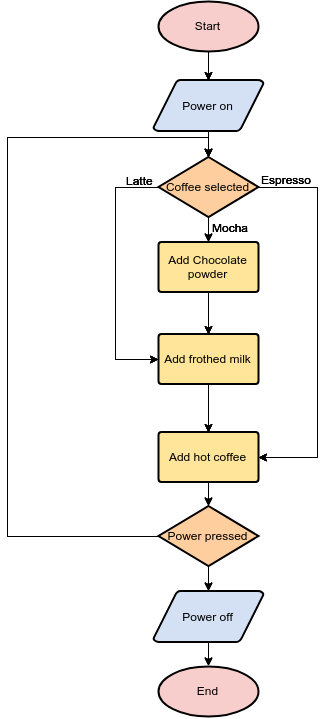
\includegraphics[width=\textwidth]{images/cm-flowchart.png}
%     }
%     \col[0.27]{
%       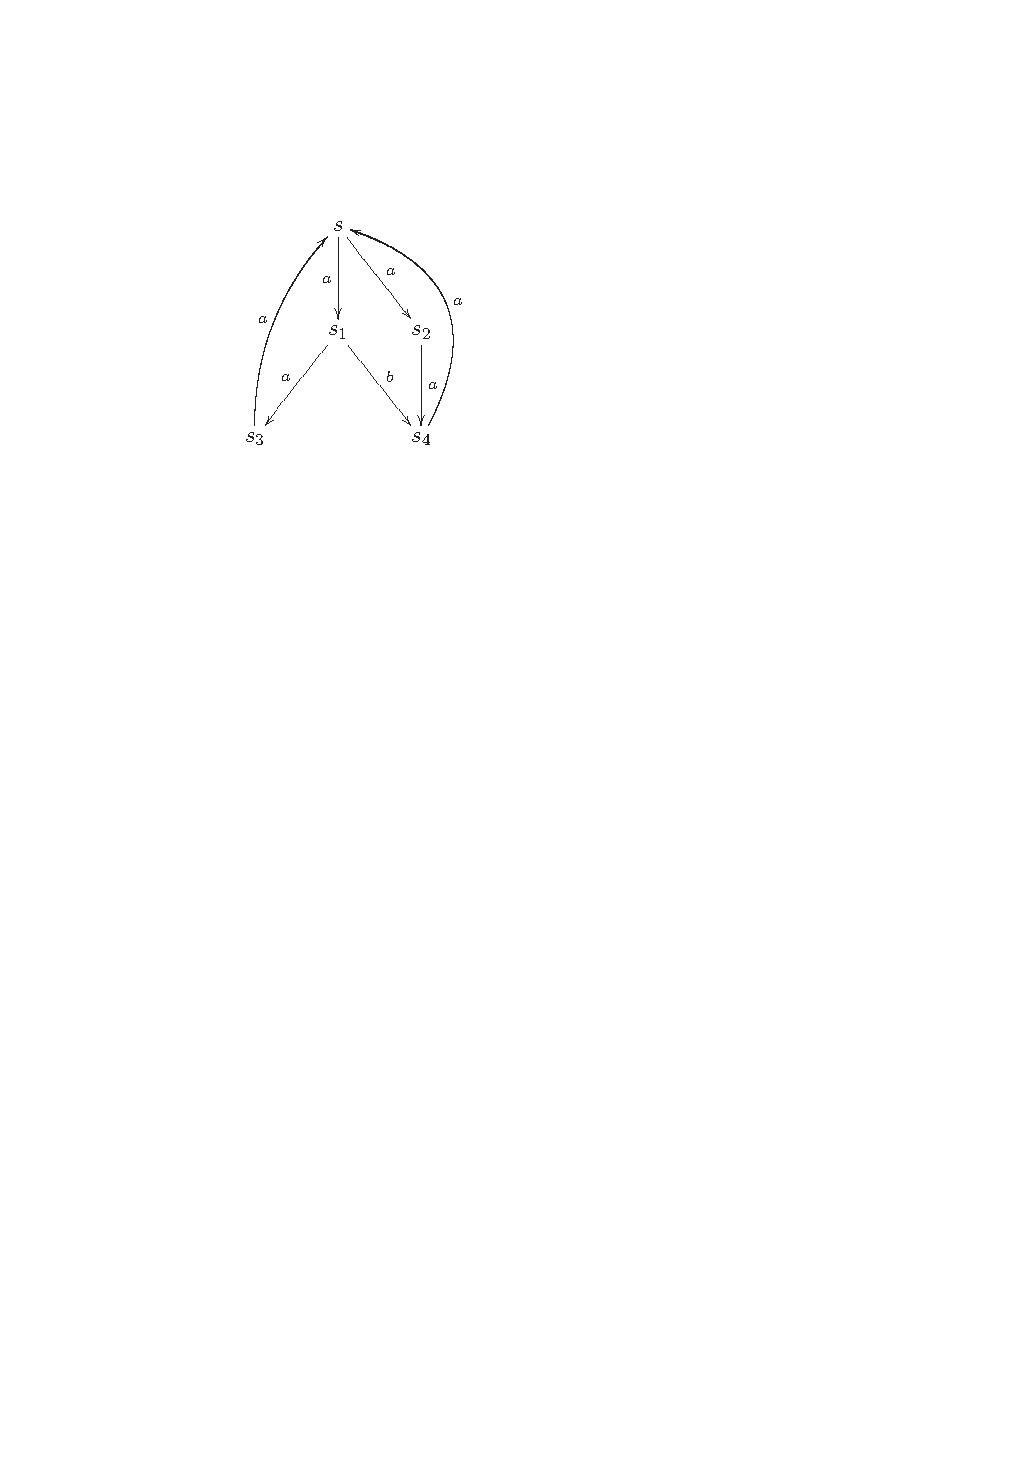
\includegraphics[width=\textwidth]{images/LTS-1.pdf}
%       \\[10mm]
%       \begin{minipage}{\textwidth}
%       \scriptsize
% % \begin{lstlisting}
% CM = €.coffee'.CM;\\
% CS = pub'.€'.coffee.CS;\
% CMCS = CM || CS;
% % \end{lstlisting}       
%       \end{minipage}
%     }
%     % \begin{tikzpicture}[aut,inner sep=3pt]
%     %   \node[st,initial]  (s0) {$s_0$};
%     %   \node[st] (s1) [right of=s0]  {$s_1$};
%     %   \node[st,final] (s2) [right of=s1]  {$s_2$}; 
%     %   \path[->] (s0) edge  node {a}  (s1)
%     %             (s1) edge[bend left]  node {b}  (s2)
%     %             (s2) edge[bend left]  node {b}  (s1);
%     %             % (s_2) edge  [loop above]  node {b}  ();
%     % \end{tikzpicture}
%   \end{columns}
  
% \end{slide}


\begin{slide}{Overview}
\begin{block}{So far}
\begin{itemize}
  \item Class diagrams, boolean and 1st order logic, ...
\end{itemize}
\end{block}

\begin{block}{Next}
\begin{itemize}
  % \item What do they mean - \alert{precisely}?
  % \item Introduction to \alert{formal methods}
  \item Look at UML \alert{behaviour} diagrams
  \item Use a domain with a \alert{precise semantics}
  \begin{itemize}
    \item Non-deterministic finite \structure{automata} (NFA)
    \item Simple language for \structure{processes}
    \item Encode processes $\to$ NFA
    \item Equivalence of processes
  \end{itemize}
\end{itemize}
\end{block}

\wrap{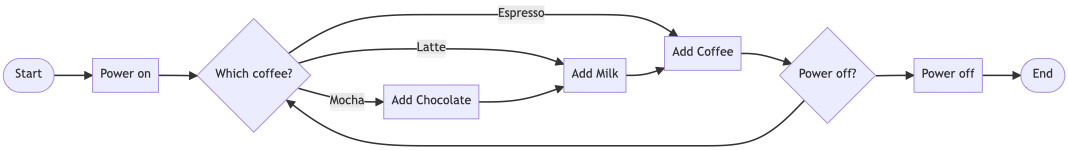
\includegraphics[width=0.7\textwidth]{images/diagrams/coffee-flow.png}}
~~
\wrap{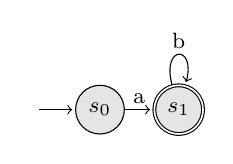
\begin{tikzpicture}[aut,node distance=1cm,font=\footnotesize]
  \node[st,initial]  (s_0)                 {$s_0$};
  \node[st,final]                    (s_2) [right of=s_0]  {$s_1$};
% 
  \path[->]
  (s_0) edge                node {a}  (s_2)
  (s_2) edge  [loop above]  node {b}  ();
\end{tikzpicture}}

\end{slide}


\begin{slide}{What are formal methods?}
  \centering

  \begin{minipage}{0.7\textwidth}
  \Large
  \begin{block}{}
    \centering
    Formal methods are \structure{techniques} to
    \\
    model \alert{complex systems} using
    \\
    \alert{rigorous mathematical models}

  \end{block}
  \end{minipage}
  \\[10mm]

  \begin{minipage}{0.32\textwidth}
  \begin{alertblock}{Specification}
    Define part of the system using a modelling language
  \end{alertblock}
  \end{minipage}
~~
  \begin{minipage}{0.3\textwidth}
  \begin{alertblock}{Verification}
    Prove properties.\\Show correctness.\\Find bugs.
  \end{alertblock}
  \end{minipage}
~~
  \begin{minipage}{0.28\textwidth}
  \begin{exampleblock}{Implementation}
    Generate correct code.\\
  \end{exampleblock}
  \end{minipage}

\end{slide}

\begin{frame}
  \huge\centering
  All formal models are \alert{wrong}
  \pause
  \\[5mm]
  ... but some of them are \structure{usefull}!
\end{frame}


% \begin{slide}{Many success cases}
%   \huge\centering

%   Cryptographic protocols
%   \\[5mm]
%   Distributed systems do not get stuck
%   \\[5mm]
%   Safety in railway systems
%   \\[5mm]
%   Type systems
%   \\[5mm]
%   \faded{\emph{[Tests: Validation (not Verification)]}}

% \end{slide}


\begin{slide}{Syllabus}
  \begin{block}{}
    TODO
  \end{block}
  \begin{itemize}
    \faded{
    \item \structure{Introduction to MDE: Visual Paradigm \& SysML}
    \item \structure{SysML: Structural and Behavioural Diagrams I}
    }
    \item {\Large \textbf{\alert{Formalisation: Sequential process algebra}}}
    \faded{
    \item \structure{SysML: Behaviour Diagrams II}
    \item \alert{Formalisation: Concurrent process algebra}
    \item \alert{Formalisation: Modelling with mCRL2}
    \item \structure{SysML: Requirements Diagram}
    \item \alert{Formalisation: Dynamic Logic \& Verification}
    \item \structure{Standards and use cases in critical systems}
    }
  \end{itemize}
\end{slide}


\section{UML behaviour diagrams}
%----------------------------------------------------------------------------------

\begin{slide}{UML behaviour diagrams}
  Describe the \structure{state} of a component, what \structure{actions} it can do, and how it \structure{evolves} during its life cycle.

  ~\\[5mm]

  \begin{itemize}
    \item \alert{State Diagram} focus on states
    \item \alert{Flow Chart} focus on actions (also known as \emph{activity diagrams})
  \end{itemize}
\end{slide}


\begin{slide}{Coffee State Diagram}
  % \begin{block}{State Diagram}
    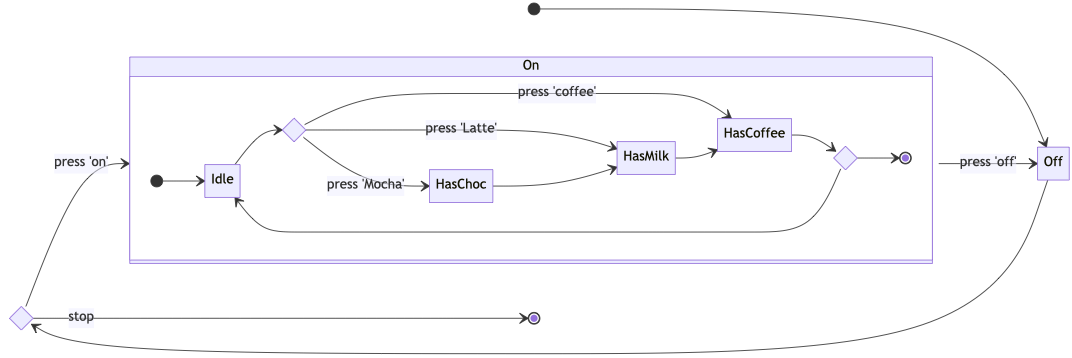
\includegraphics[width=1.0\textwidth]{images/diagrams/coffee-state.png}
  % \end{block}
\end{slide}

\begin{slide}{Coffee Flow Chart}
  % \begin{block}{Flow Chart}
    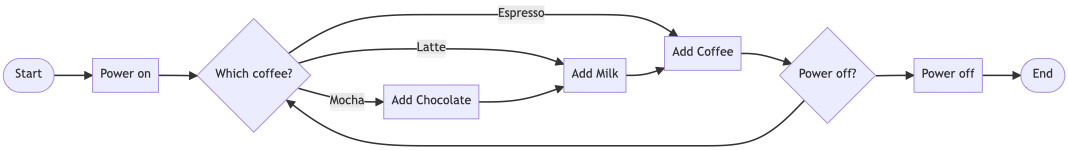
\includegraphics[width=1.0\textwidth]{images/diagrams/coffee-flow.png}
  % \end{block}
  \\[6mm]
  \frsplitt{
  \structure{Used symbols}: \emph{processes}, \emph{decisions}, and \emph{start/end}
  }{
  \structure{Other symbols} include: data (or input/output), documents, connectors, comments
  }
\end{slide}


\section{Automata -- Basic definitions}
%----------------------------------------------------------------------------------
\begin{slide}{Sequential and Reactive systems}
% \small

\frsplitt{\begin{block}{Sequential systems}
~\\[1mm]
Meaning is defined by the results of finite computations
\\[1mm]~
\end{block}}{
\begin{block}{Reactive systems}
~\\[1mm]
Meaning is determined by \structure{interaction} and \structure{mobility} of \structure{non-terminating} processes, 
evolving \structure{concurrently}
\\[1mm]~
\end{block}}

\bigskip

\frsplitt{\alert{This module}}{\alert{The next module}}


% \begin{block}{Reactive system}
% Meaning determined by \structure{interaction} and \structure{mobility} of \structure{non-terminating} processes, 
% evolving \structure{concurrently}
% \end{block}
% \caixa{system that computes by reacting to stimuli from its environment along its overall computation}
% \begin{itemize}
% \item in contrast to sequential systems whose meaning is defined by the results of finite computations, the behaviour of reactive systems is mainly determined by \structure{interaction} and \structure{mobility} of \structure{non-terminating} processes, 
% evolving \structure{concurrently}.
% \item \structure{observation} $\; \equiv\;$ interaction
% \item \structure{behaviour} $\; \equiv\;$ a structured record of interactions
% \end{itemize}
\end{slide}

%----------------------------------------------------------------------------------
\begin{slide}{Non-Deterministic Finite Automata (NFA)}
\small
\begin{block}{Definition}
A NFA over a set $\Act$ of names is a tuple
$\pair{S, I, \downarrow, \Act,  \rra}$ where
\begin{itemize}
\item $S = \enset{s_0, s_1, s_2, ...}$ is a set of states
\item $I \subseteq S$ is the set of \structure{initial} states
\item  $\downarrow \subseteq S$ is the set of \structure{terminating} or final states
\begin{equation*}
\downarrow s \; \equiv\; s \in \downarrow
\end{equation*}
\item  $\rra \,\,\subseteq\, S \times \Act \times S$ is the \structure{transition} relation, often given as an $\Act$-indexed family of binary relations 
\begin{equation*}
s \rtran{a} s'\; \equiv\; \pair{s,a,s'} \in \rra
\end{equation*}
\end{itemize}
\end{block}
\end{slide}


\begin{slide}{Example}
  \begin{block}{Example of an automaton}
  \centering
  \wrap{
  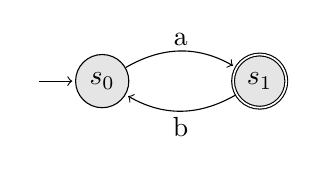
\begin{tikzpicture}[aut]
    \node[st,initial]  (s_0)                 {$s_0$};
    \node[st,final]  (s_1) [right of=s_0]  {$s_1$};
  % 
    \path[->]
    (s_0) edge[bend left] node {a}  (s_1)
    (s_1) edge[bend left] node {b}  (s_0);
  \end{tikzpicture}
  }
  ~~~~
  \wrap{$s_0$ is an initial state\\$s_1$ is a final state} 
  \end{block}
  %
  ~\\[0mm]
  %
  \begin{block}{}
    \faded{(Formalise this automata)}
      \\[0.25\textheight]
  \end{block}

\end{slide}


\begin{slide}{Exercise}
\doExercise{Formalise these automata as $\pair{S,I,\dda,\Act,\rra}$}{
\centering
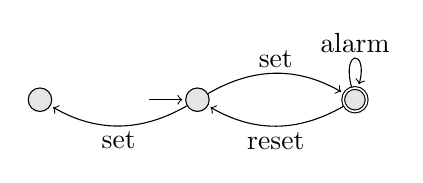
\begin{tikzpicture}[aut]
  \node[st] (s_0) {};
  \node[st,initial,right of=s_0] (s_1) {};
  % \node[st] (s_2) [right of=s_1]  {};
  \node[st,final] (s_2) [right of=s_1]  {};
% 
  \path[->]
  (s_1) edge[bend left] node {set} (s_2)
  (s_1) edge[bend left] node{set} (s_0)
  (s_2) edge  [loop above]  node {alarm} () edge[bend left] node{reset} (s_1);
\end{tikzpicture}
~~~~~~~~~~
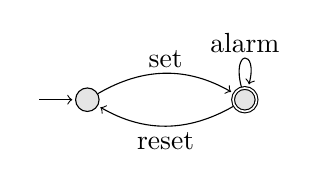
\begin{tikzpicture}[aut]
  \node[st,initial] (s_1) {};
  \node[st,final] (s_2) [right of=s_1]  {};
% 
  \path[->]
  (s_1) edge[bend left] node {set} (s_2)
  (s_2) edge  [loop above]  node {alarm} () edge[bend left] node{reset} (s_1);
\end{tikzpicture}

}
  
\end{slide}



    % 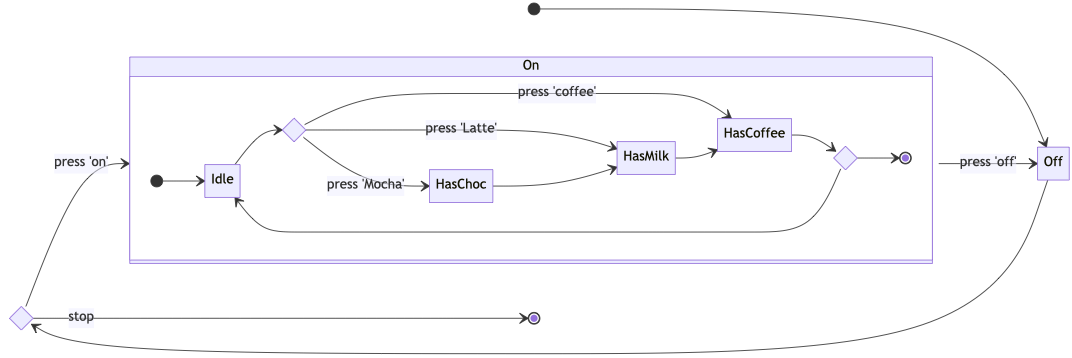
\includegraphics[width=1.0\textwidth]{images/diagrams/coffee-state.png}

\begin{slide}{Exercise}
  \centering

  \vspace{-1mm}
  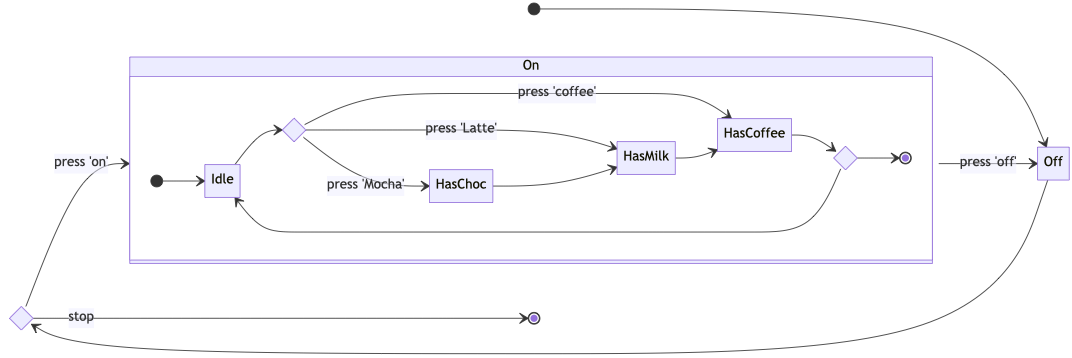
\includegraphics[width=1.0\textwidth]{images/diagrams/coffee-state.png}
  \vspace{-1mm}

  \doExercise{Draw LTS}{
      \faded{(suggestion: by hand on a paper, and take a photo of it.)}
      \\[0.30\textheight]
  }
\end{slide}


% \begin{slide}{Exercise}
%   \centering

%   \vspace*{-2mm}
%   \begin{columns}
%     \column{0.40\textwidth}\centering
%     \begin{block}{Flowchart}
%       \centering
%       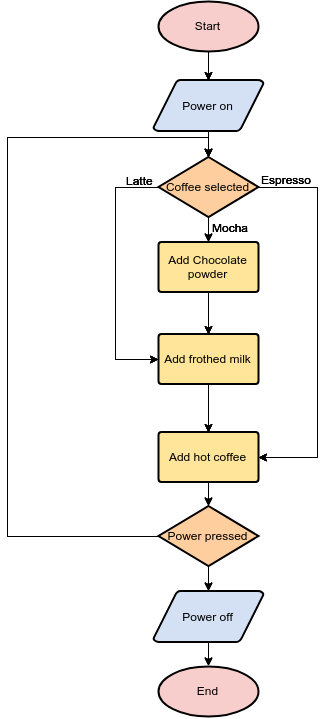
\includegraphics[height=0.85\textheight]{images/cm-flowchart.png}
%     \end{block}
%     \column{0.56\textwidth}\centering
%     \doExercise{Draw LTS}{
%       \faded{(suggestion: by hand on a paper, and take a photo of it.)}
%       \\[0.75\textheight]
%     }
%   \end{columns}
% \end{slide}

%----------------------------------------------------------------------------------
% \begin{slide}{Labelled Transition System}
% \small
% \begin{block}{Morphism}
% A \structure{morphism} relating two LTS over  $\Act$, $\pair{S,\Act, \rra}$ and $\pair{S',\Act,  \rra'}$,
% is a function $\fdec{h}{S}{S'}$  st
% \begin{align*}
% s \rtran{a} s' \; \; \; \; \;  \imp & \; \; \; \; \; \apf{h}{s}  \primertran{a} \apf{h}{s'} 
% \end{align*}
% \end{block}

% \begin{center}
% \fbox{morphisms \structure{preserve} transitions}
% \end{center}
% \end{slide}

%----------------------------------------------------------------------------------
\begin{slide}{Labelled Transition System}
\small
% \begin{block}{System}
% Given an automaton $\pair{S, I, \dda, \Act, \rra}$, each state $s \in S$ determines a \structure{system} over 
% all states reachable from $s$ and the corresponding restriction of $\rra$.
% % and $\downarrow$.
% \end{block}

More generally, a NFA $\pair{S,I,\dda,\Act,\rra}$ is a \structure{labelled transition system} (LTS) $\pair{S,\Act,\rra}$, where each state $s \in S$ determines a \structure{system} over all states reachable from $s$ and the corresponding restriction of $\rra$.

\begin{block}{LTS classification}
\begin{itemize}
\item \alert{deterministic}
\item \alert{non deterministic}
\item \alert{finite}
\item \alert{finitely branching}
\item \alert{image finite}
\item ...
\end{itemize}
\end{block}

\end{slide}


%----------------------------------------------------------------------------------
% \begin{slide}{Language of an Automaton}
% \small

% Let $A = \pair{S, I, \dda, \Act,  \rra}$ be a NFA.

% \begin{block}{Transitive closure $\rra^{*}$}
% Let $N^{*}$ denote the set of all \structure{words} $a_1a_2\ldots a_n$, where $a_i \in N$ and $n \geq 0$. 
% The \alert{transitive closure} ${\rra^{*}} \subseteq S \times N^{*} \times S$, denoting $s\rtrant{w}s' \; \equiv\; (s,w,s') \in \rra^{*}$, be the minimal set satisfying:
% \begin{align*}
% \text{\alert{(1)}}\; \;  & 
%   s\in S \;\imp\; s \rtrant{\epsilon} s
%   % \rcb{\forall}{s}{s \in S}{s \rtrant{\epsilon} s}\\
% %
% \text{\alert{(2)}}\; \;  &
%   s \rtrant{w} s' \land s' \rtran{a} s'' \; \imp\;  s \rtrant{wa} s''
% %
% % \text{\alert{(2)}}\; \;  & 
%   % s \sigma \in \Tr{s}\; \imp\; \rcb{\exists}{s'}{s' \in S}{s \rtran{a} s'\, \e\, \sigma \in \Tr{s'}}
% \end{align*}


%----------------------------------------------------------------------------------
\begin{slide}{Reachability}
\small
\begin{block}{Definition}
The \structure{reachability relation}, ${\rra^*} \subseteq S \times \Act^* \times S$, is defined inductively
\begin{itemize}
\item $s \reach{\!\!\!\!\!\epsilon} s$ for each $s \in S$, where $\epsilon \in \Act^*$ denotes the empty \alert{word};
\item if  $s \rtran{a} s''$  and $s'' \reach{\!\!\!\!\!\sigma} s'$ then $s \reach{\!\!\!\!\!a \sigma} s'$, for $a \in \Act, \sigma \in \Act^*$
\end{itemize}
\end{block}

\begin{block}{Reachable state}
$t \in S$ is \structure{reachable} from $s \in S$ iff there is a \alert{word} $\sigma \in \Act^*$ st $s \reach{\!\!\!\!\!\sigma} t$
\end{block}

\end{slide}

\begin{slide}{Language of an Automaton}
\small

% Let $A = \pair{S, I, \dda, \Act,  \rra}$ be a NFA.

% \begin{block}{Transitive closure $\rra^{*}$}
% Define ${\rra^{*}} \subseteq S \times N^{*} \times S$ to be the \structure{transitive closure} of $\rra$ defined as the minimal set such that:
% \begin{align*}
% \text{\alert{(1)}}\; \;  & 
%   s\in S \;\imp\; (s,\epsilon,s) \in {\rra^{*}}\\  
% \text{\alert{(2)}}\; \;  &
%   (s,w,s') \in {\rra^{*}} ~\land~ s' \rtran{wa} s'' ~~\imp~~  (s,\epsilon,s'') \in {\rra^{*}}
% \end{align*}
% \end{block}

% Notation: $s\rtrant{w}s' \; \equiv\; (s,w,s') \in {\rra^{*}}$

\begin{block}{Language}
  \centering
  % The \structure{language $L_A$} of $A$ is the smallest set such that:
  % \begin{align*}
  %   s \in I ~\land~ s'\dda ~\land~ s\rtrant{w} s' ~~\imp~~ w \in L_A
  % \end{align*}
  A word $\sigma$ is in the \structure{language $L_A$} of an automata $A = \pair{S,I,\dda,N,\rra}$
  \\iff\\
  there are states $s\in I$, $s' \in \dda$ such that $s\rtrant{\sigma}s'$.
\end{block}
\end{slide}



\begin{slide}{Exercises}
\doExercise{What is the language of this automata?}{
\centering
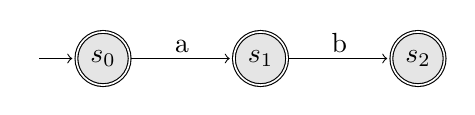
\begin{tikzpicture}[aut]
  \node[st,initial,final]  (s_0)                 {$s_0$};
  \node[st,final]                    (s_1) [right of=s_0]  {$s_1$};
  \node[st,final]                    (s_2) [right of=s_1]  {$s_2$};
% 
  \path[->]
  (s_0) edge                node {a}  (s_1)
  (s_1) edge                node {b}  (s_2);

\end{tikzpicture}
}

\doExercise{What is the language of this automata?}{
\centering
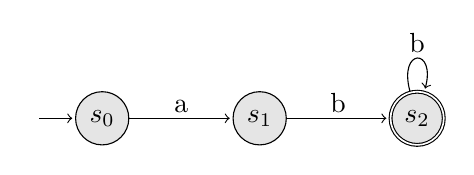
\begin{tikzpicture}[aut]
  \node[st,initial]  (s_0)                 {$s_0$};
  \node[st]                    (s_1) [right of=s_0]  {$s_1$};
  \node[st,final]                    (s_2) [right of=s_1]  {$s_2$};
% 
  \path[->]
  (s_0) edge                node {a}  (s_1)
  (s_1) edge                node {b}  (s_2)
  (s_2) edge  [loop above]  node {b}  ();
\end{tikzpicture}
}

\doExercise{What is the language of this automata?}{
\centering
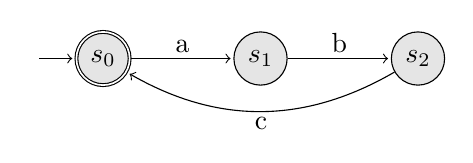
\begin{tikzpicture}[aut]
  \node[st,initial,final]  (s_0)                 {$s_0$};
  \node[st]                    (s_1) [right of=s_0]  {$s_1$};
  \node[st]                    (s_2) [right of=s_1]  {$s_2$};
% 
  \path[->]
  (s_0) edge                node {a}  (s_1)
  (s_1) edge                node {b}  (s_2)
  (s_2) edge[bend left] node {c}  (s_0);
\end{tikzpicture}
}

\end{slide}




%----------------------------------------------------------------------------------
%\begin{slide}{An alternative characterisation}
%\small
%\begin{block}{Coalgebraic  characterization (morphism)}
%A \structure{morphism} $\fdec{h}{\pair{S, \nx}}{\pair{S', \nx'}}$ is a function 
%$\fdec{h}{S}{S'}$ st the following diagram commutes
%\begin{equation*}
%\xymatrix{
%S \times \Act \ar[d]_-{h \times \id} \ar[r]^-{\nx} & \ppow{S} \ar[d]^-{\ppow{h}}\\
%S' \times \Act \ar[r]^-{\nx'} & \ppow{S'}
%}
%\end{equation*}
%i.e.,
%\begin{equation*}
%\ppow{h} \comp \nx\; \; =\; \; \nx' \comp (h \times \id)
%\end{equation*}
%or, going pointwise,
%\begin{equation*}
%\setdef{\apf{h}{x}}{x \in \apf{\nx}{\pair{s,a}}}\; \;   =\; \;  \apf{\nx'}{\pair{\apf{h}{s},a}} 
%\end{equation*}
%\end{block}
%\end{slide}
%
%%----------------------------------------------------------------------------------
%\begin{slide}{An alternative characterisation}
%\small
%\begin{block}{Coalgebraic  characterization (morphism)}
%A \structure{morphism} $\fdec{h}{\pair{S, \nx}}{\pair{S', \nx'}}$ 
%\begin{itemize}
%\item \structure{preseves} transitions:
%\begin{equation*}
%s' \in \apf{\nx}{\pair{s,a}} \imp \apf{h}{s'} \in \apf{\nx'}{\pair{\apf{h}{s},a}} 
%\end{equation*}
%\item \structure{reflects} transitions:
%\begin{equation*}
%r' \in \apf{\nx'}{\pair{\apf{h}{s},a}} \imp \rcb{\exists}{s' \in S}{s' \in \apf{\nx}{\pair{s,a}}}{r' = \apf{h}{s'}}  
%\end{equation*}
%\end{itemize}
%\end{block}
%\alert{(why?)}
%\end{slide}
%
%
%%----------------------------------------------------------------------------------
%\begin{slide}{Comparison}
%\small
%
%\begin{itemize}
%\item Both definitions coincide at the \alert{object} level:
%\begin{equation*}
%\pair{s,a,s'} \in T\; \; \equiv\;\; s' \in \apf{\nx}{\pair{s,a}}
%\end{equation*}
%\item Wrt \alert{morphisms}, the relational definition is more general, corresponding, in coalgebraic terms to
%\begin{equation*}
%\ppow{h} \comp \nx\; \; \subseteq\; \; \nx' \comp (h \times \id)
%\end{equation*}
%\end{itemize}
%
%
%\pause
%
%%\begin{alertblock}
%\myblock{How can these notions of \structure{morphism} be used to compare LTS?}
%%\end{alertblock}
%
%
%\end{slide}


\section{Process algebra}

%-------------------------------------------------------------------------------
\begin{slide}{Process algebras}
\small

\begin{block}{CCS - Syntax}
\begin{equation*}
\mathcal{P} ~\ni~ P,Q\; ::=\; K ~~|~~ \alpha.P ~~|~~ \sum_{i\in I} P_i
        ~~|~~ \crn P f \transp{~~|~~ P|Q ~~|~~ P\backslash L}
\end{equation*}
%
where
\\- $\alpha \in \Act \transp{\cup \overline\Act \cup \set{\tau}} $~ is an action
\\- $K$ s a collection of process names or process contants
\\- $I$ is an indexing set
\\- $L \subseteq \Act \transp{\cup \overline{\Act}}$ is a set of labels
\\- $f$ is a function that renames actions s.t. $f(\tau) = \tau$ and $f(\overline{a}) = \overline{f(a)}$
\\- notation:
\\~~~~~$\cnil = \sum_{i\in\emptyset}P_i$
\\~~~~~$P_1+P_2 = \sum_{i\in\set{1,2}}P_i$
\\~~~~~$[f] = [b_1/a_1,\ldots,b_n/a_n]$
\end{block}
\end{slide}

%-------------------------------------------------------------------------------

\begin{slide}{Process algebras}
\small

\begin{block}{Syntax}
\begin{equation*}
\mathcal{P} ~\ni~ P,Q\; ::=\; K ~~|~~ \alpha.P ~~|~~ \sum_{i\in I} P_i
    ~~|~~ \crn P f \transp{~~|~~ P|Q ~~|~~ P\backslash L}
\end{equation*}
\end{block}

%\setcounter{equation}{0}
\begin{exampleblock}{Exercise: Which are syntactically correct?}
\frsplit[.40]{
\begin{align}
  & a.b.A+B\\&
  (a.\cnil + \ainv a.A) \backslash \set{a,b}\\&
  (a.\cnil + \ainv a.A) \backslash \set{a,\tau}\\& % no
  a.B+[a/b]\\& % no
  \tau.\tau.B + \cnil\\&
  (a.B + b.B)[a/a,b/\tau]
\end{align}
}{\begin{align} &
  (a.B + \tau.B)[a/b,a/a]\\& % no
  (a.b.A + \ainv a.\cnil)|B\\&
  (a.b.A + \ainv a.\cnil).B\\&
  (a.b.A + \ainv a.\cnil)+B\\&
  (\cnil | \cnil) + \cnil
\end{align}
}
\end{exampleblock}

\end{slide}

%-------------------------------------------------------------------------------

\begin{slide}{CCS semantics - building an LTS}
\small 
\centering
\newcommand{\msep}{~~~~~~}

\typerule{act}{\shrk}{\alpha.P \trans\alpha P}
\msep
\typerule{sum-j}{P_j \trans\alpha P'_j}{\sum_{i\in I}P_i \trans\alpha P'_j} $\transp{j\in I}$
\\[3mm]
\typerule{com1}{P\trans\alpha P'}{P|Q\trans\alpha P'|Q}
\msep
\typerule{com2}{Q\trans\alpha Q'}{P|Q\trans\alpha P|Q'}
\msep
\typerule{com3}{P\trans a P' \quad Q\trans{\ainv{a}} Q'}{P|Q\trans\tau P'|Q'}
\\[3mm]
\typerule{res}{P\trans\alpha P'}{\crt P L\trans\alpha \crt{P'}L}~$\transp{\alpha,\ainv{\alpha} \notin L}$
\msep
\typerule{rel}{P\trans\alpha P'}{\crn P f\trans{f(\alpha)} \crn{P'} f}
\\[2mm]
\pause

\begin{exampleblock}{Exercise: Draw the LTS's}
  \vspace*{-4mm}
  \begin{align*}
    CM &= \mathsf{coin.\ainv{coffee}}.CM
    \\
    CS &= \mathsf{\ainv{pub}.\ainv{coin}.coffee}.CS
    \\
    SmUni &= \crt{(CM|CS)}{\mathsf{\set{coin,coffee}}}
  \end{align*}
\end{exampleblock}

\end{slide}

%-------------------------------------------------------------------------------
\begin{slide}{mCRL2}
\small
\myblock{\url{http://mcrl2.org}}
  
\begin{itemize}
  \item {Formal \structure{specification language} with an associated toolset}
  
  \item {Used for \structure{modelling}, \structure{validating} and \structure{verifying} concurrent systems and protocols}
\end{itemize}
  
\end{slide}

%-------------------------------------------------------------------------------
\begin{frame}[fragile]{mCRL2}
  
\begin{block}{Syntax (by example)}
\begin{align*}
  a.P &\to \mcode{a.P}
  \\
  P_1 + P_2 &\to \mcode{P1 + P2}
  \\
  P\backslash L &\to \mcode{block(L,P)}
 \\
 \crn{P}{f} &\to \mcode{rename(f,P)}
  \\
  a.P|\ainv a.Q &\to \mcode{hide(\{a\},}\mcode{comm(\{a1|a2->a\}, }\mcode{a1.P}\mcode{||a2.P))}
  \\
  a.P|\ainv a.Q \backslash \{a\}  &\to \mcode{hide(\{a\},}\mcode{block(\{a1,a2\},}\mcode{comm(\{a1|a2->a\}, }
  \\&~~~~~
  \mcode{a1.P}\mcode{||a2.Q)))}
\end{align*}
\end{block}
\end{frame}

%-------------------------------------------------------------------------------
\begin{frame}[fragile]{mCRL2}
\small
%  \myblock{\url{http://mcrl2.org}}
  
%  \begin{block}{Syntax (by example)}

\begin{lstlisting}
act
  coin, coin', coinCom,
  coffee, coffee', coffeeCom, pub';

proc
  CM = coin.coffee'.CM;
  CS = pub'.coin'.coffee.CS;
  CMCS = CM || CS;
  SmUni = hide({coffeeCom,coinCom},
          block({coffee,coffee',coin,coin'},
          comm({coffee|coffee' -> coffeeCom,
                coin|coin'     -> coinCom},
          CMCS )));
init
  SmUni;
\end{lstlisting}
%  \end{block}
\end{frame}

%-------------------------------------------------------------------------------
\begin{slide}{mCRL2 toolset overview}
  \centering
  
  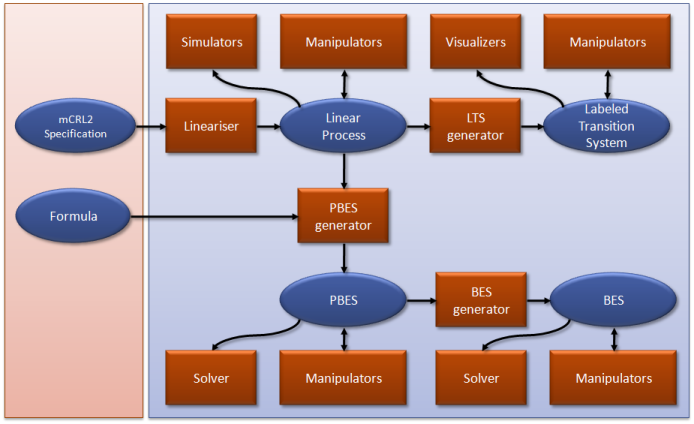
\includegraphics[width=\textwidth]{images/mcrl2-toolset.png}

  -- mCRL2 tutorial: Modelling part --
\end{slide}

%-------------------------------------------------------------------------------
\section{Behavioural equivalences}

%----------------------------------------------------------------------------------
\begin{slide}{Behavioural Equivalences -- Intuition}
\small


Two LTS should be \structure{equivalent} if they cannot be distinguished by interacting with them.


\begin{block}{Equality of functional behaviour}
is not preserved by \alert{parallel} composition: non \alert{compositional} semantics, cf,
\begin{center}
\texttt{x:=4; x:=x+1} ~and~ \texttt{x:=5}
\end{center}
\end{block}

\begin{block}{Graph isomorphism} 
is too strong (why?)
\end{block}

\end{slide}



%----------------------------------------------------------------------------------
\begin{slide}{Trace}
\small

\begin{block}{Definition}
Let $T = \pair{S, \Act,  \rra}$ be a labelled transition system. The set of \structure{traces} $\Tr{s}$, for $s \in S$ is the minimal set  satisfying
\begin{align*}
\text{\alert{(1)}}\; \;  &  \epsilon \in \Tr{s}\\
\text{\alert{(2)}}\; \;  &  a \sigma \in \Tr{s}\; \imp\; \rcb{\exists}{s'}{s' \in S}{s \rtran{a} s'\, \e\, \sigma \in \Tr{s'}}
\end{align*}
\end{block}


\end{slide}

%----------------------------------------------------------------------------------
\begin{slide}{Trace  equivalence}
\small

\begin{block}{Definition}
Two states $s, r$ are \structure{trace equivalent} iff  $ \Tr{s} =  \Tr{r}$\\
(i.e. if they can perform the same finite sequences of transitions)
\end{block}
~\\

\begin{example}
  \centering
  % Requires \usepackage{graphicx}
  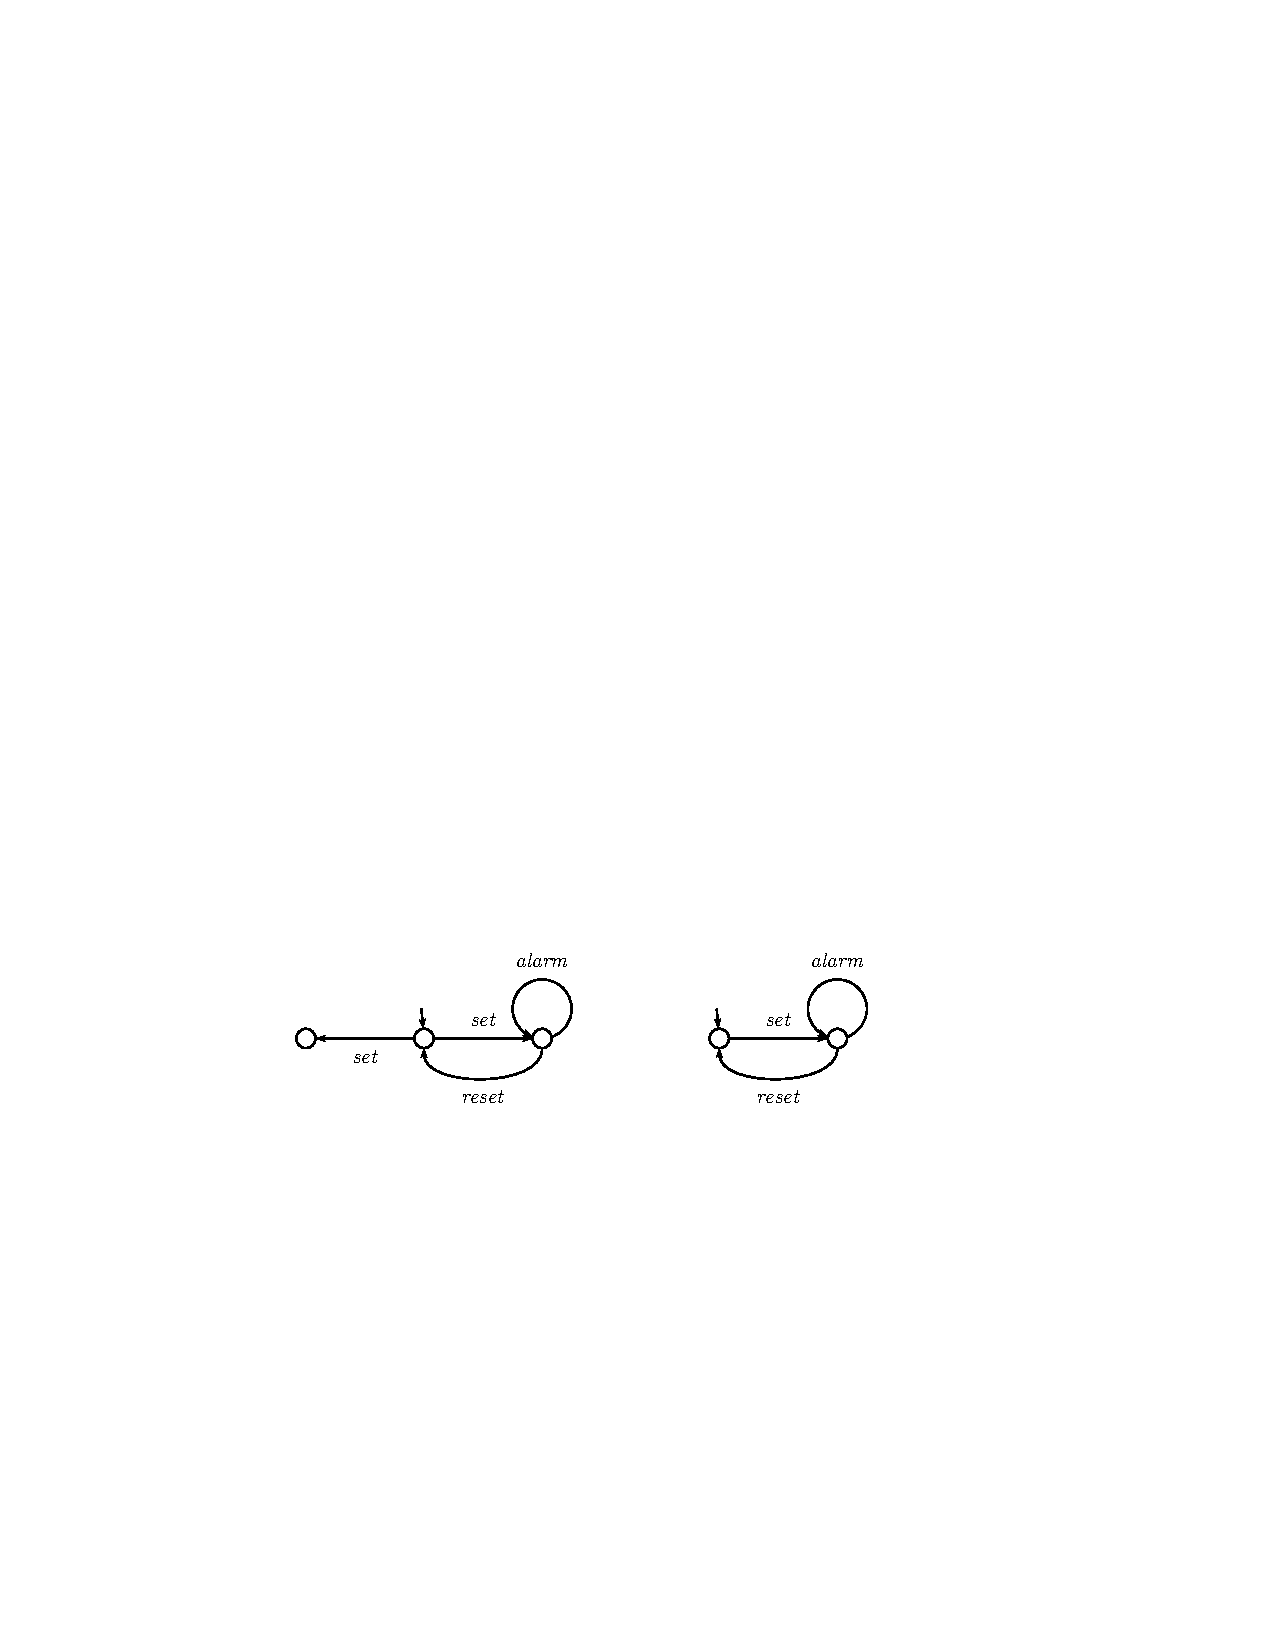
\includegraphics[width=9cm]{./images/alarm3.pdf}
\end{example}


\alert{Trace equivalence} applies  when one can neither interact with a system, nor distinguish a slow system from one that has come to a stand still.
\end{slide}



\section{Similarity}

%----------------------------------------------------------------------------------
\begin{slide}{Simulation}
\begin{flushright}
the quest for a \structure{behavioural equality}:\\
able to identify states that cannot be distinguished by any \structure{realistic} form of  observation
\end{flushright}
~\\

\small
\begin{block}{Simulation}
\caixa{A state $q$ \structure{simulates} another state $p$
\structure{if}\\
every transition from $q$ is corresponded by a transition from $p$
\structure{and}\\
this capacity is kept along the whole life of the system to which state space $q$ belongs to.}
\end{block}
\end{slide}

%----------------------------------------------------------------------------------
\begin{slide}{Simulation}
\small

\begin{block}{Definition}
Given  $\pair{S_1, \Act, \rra_1}$  and $\pair{S_2, \Act, \rra_2}$
 over $\Act$,
relation \structure{$R \subseteq S_1 \times S_2$} is a \structure{simulation} iff,
for all $\pair{p,q} \in \structure{R}$ and $a \in \Act$,

\begin{align*}
%\text{\alert{(1)}}\; \;  & p \downarrow_1 \;  \imp\; q \downarrow_2\\ &\\
\text{\alert{(1)}}\; \;  & p \rtran{a}_1 p'\;  \imp\; \rcb{\exists}{q'}{q' \in S_2}{q \rtran{a}_2 q'\, \e\, \pair{p',q'} \in \structure{R}}   
\end{align*}
\vspace{6mm}

\begin{equation*}
\xymatrix{
p \ar[d]^-{a} & \hspace{-1.5cm} \structure{R}  & \hspace{-2.7cm} q 
  & \!\! \text{\raisebox{-10mm}{\Huge $\imp$}} \! \! &  &  &  q \ar[d]^-{a} \\
p'           &   &           &                                   & p'\hspace{-2.7cm} &  \structure{R} \hspace{-1.5cm} &  q'
}
\end{equation*}

\end{block}
\end{slide}

%----------------------------------------------------------------------------------
\begin{slide}{Example}

\begin{exampleblock}{Find simulations}
\begin{equation*}
\xymatrix{
& q_1  \ar[r]^{d} & q_2 &       &        &                              p_2\\
q_0 \ar[ru]^{a} \ar[rd]_{a} &  & & p_0 \ar[r]^{a} & p_1 \ar[ru]^{d} \ar[rd]_{e} & \\
& q_4  \ar[r]_{e} & q_3 &       &        &                              p_3\\
}
\end{equation*}
\end{exampleblock}

\vspace{0.2cm}
\visible<2->{\begin{equation*}
q_0 \lesssim p_0 \text{\hspace{0.5cm} cf. \hspace{0.3cm}} 
\enset{\pair{q_0,p_0}, \pair{q_1,p_1},\pair{q_4,p_1},\pair{q_2,p_2},\pair{q_3,p_3}}
\end{equation*}}
\end{slide}

%----------------------------------------------------------------------------------
\begin{slide}{Similarity}
\small

\begin{block}{Definition}
\centering
\[p \lesssim q\; \equiv\; \rcb{\exists}{R}{}{R\; \text{is a simulation and}\; \pair{p,q} \in R} 
\]
\emph{We say \structure{$q$ simulates $p$}.}
\end{block}
\begin{block}{Lemma}
The similarity relation is a preorder\\
\transp{(ie, reflexive and transitive)}
\end{block}
\end{slide}


\section{Bisimilarity}
%----------------------------------------------------------------------------------
\begin{slide}{Bisimulation}
\small

\begin{block}{Definition}
Given  $\pair{S_1, \Act,  \rra_1}$  and $\pair{S_2, \Act, \rra_2}$ over $\Act$,
relation $R \subseteq S_1 \times S_2$ is a \structure{bisimulation} iff both $R$ and its converse $\aconv{R}$
are simulations.

I.e.,
whenever $\pair{p,q} \in R$ and $a \in \Act$,

\begin{align*}
%\text{\alert{(1)}}\; \;  &  p \downarrow_1 \;  \dimp\; q \downarrow_2\\ &\\
\text{\alert{(1)}}\; \;  & p \rtran{a}_1 p'\; \imp\; \rcb{\exists}{q'}{q' \in S_2}{q \rtran{a}_2 q'\, \e\, \pair{p',q'} \in R}   \\
\text{\alert{(2)}}\; \;  & q \rtran{a}_2 q'\; \imp\; \rcb{\exists}{p'}{p' \in S_1}{p \rtran{a}_1 p'\, \e\, \pair{p',q'} \in R}   
\end{align*}

%\begin{equation*}
%\xymatrix{
%p \ar[d]^-{a} & \hspace{-1.5cm} R  & \hspace{-2.7cm} q
%    & \! \! \text{\raisebox{-10mm}{\Huge $\Leftrightarrow$}} \! \! &   &  
%    &  q \ar[d]^-{a} \\
%p'           &   &           &                                   & p'\hspace{-2.7cm} &  R \hspace{-1.5cm} &  q'
%}
%\end{equation*}
\centering
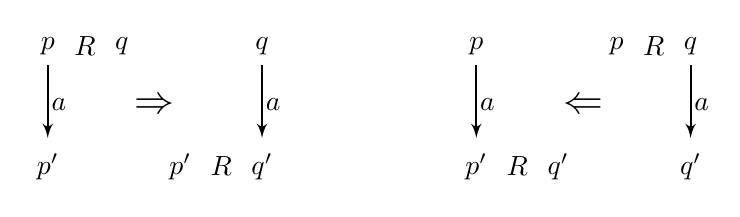
\begin{tikzpicture}[%
    every edge/.style={draw, thick,-latex',shorten >= 2pt}]
  \tikzstyle{l} = [auto,inner sep=1pt]
  % the square
  \node(p){$p$};\node[right=2.3 of p](q2){$q$};
  \node[below=1 of p](p'){$p'$};\node(q')at(p'-|q2){$q'$};
  % the R parts
  \node[right=0 of p](R1){$R$};\node[right=0 of R1](q){$q$};
  \node[left=0 of q'](R2){$R$};\node[left=0 of R2](p'2){$p'$};
  % the arrows
  \draw[->] (p)edge node[l]{$a$}(p') (q2)edge node[l]{$a$}(q');
  \node at ($(p)!.5!(q')$){{\Large $\Rightarrow$}};
  %%%%%%%
  % the square
  \node[right=2.3 of q2](pp){$p$};\node[right=2.3 of pp](q2){$q$};
  \node[below=1 of pp](p'){$p'$};\node(q')at(p'-|q2){$q'$};
  % the R parts
  \node[right=0 of p'](R1){$R$};\node[right=0 of R1](q){$q'$};
  \node[left=0 of q2](R2){$R$};\node[left=0 of R2](p'2){$p$};
  % the arrows
  \draw[->] (pp)edge node[l]{$a$}(p') (q2)edge node[l]{$a$}(q');
  \node at ($(pp)!.5!(q')$){{\Large $\Leftarrow$}};

\end{tikzpicture}

\end{block}
\end{slide}



%----------------------------------------------------------------------------------
\begin{slide}{Examples}

\begin{exampleblock}{Find bisimulations}
\begin{equation*}
\xymatrix{
& q_1  \ar[ld]_{a}  \ar[rd]^{a} & & & & m \ar[d]_{a}\\
q_2 \ar[rr]^{c}  && q_3 \ar@(ur,dr)[]^{c}  & & & n\ar@(ur,dr)[]^{c}
}
\end{equation*}
% R = \enset{(q_1,m), (q_2, n), (q_3,n) }
\vspace{1cm}

\begin{equation*}
\xymatrix{
q_1 \ar[r]^{a} & q_2  \ar[r]^{a}  & q_3  \ar[r]^{a} & \cdots & & h\ar@(ur,dr)[]^{a}  \\
}
\end{equation*}
% R = \setdef{q_i, h}{i \geq 1}  
\end{exampleblock}

\end{slide}


%----------------------------------------------------------------------------------
\begin{slide}{Examples}

\begin{exampleblock}{Find bisimulations}
\vspace*{-2mm}
\begin{equation*}
\xymatrix{
& q_1  \ar[ld]_{a}  \ar[rd]^{a} & & & & p_1  \ar[d]^{a} \\
q_2 \ar[d]^{c}  && q_3  \ar[d]^{c}  & && p_2  \ar[ld]_{c}  \ar[rd]^{c} & \\
q_4 & & q_5 & &p_4 & & p_5\\
& q_1  \ar[ld]_{a}  \ar[rd]^{a} & & & & p_1  \ar[d]^{a} \\
q_2 \ar[d]^{c}  && q_3  \ar[d]^{\rdb{b}}  & && p_2  \ar[ld]_{c}  \ar[rd]^{\rdb{b}} & \\
q_4 & & q_5 & &p_4 & & p_5
}
\end{equation*}
\end{exampleblock}
\end{slide}

%----------------------------------------------------------------------------------
\begin{slide}{After thoughts}
\small


\begin{itemize}
\item Follows a \alert{$\forall, \exists$ pattern}: $p$ in all its transitions challenge $q$ which is called to find a match to each of those (and conversely)
\item Tighter correspondence with transitions
\item Based on the information that the transitions convey, rather than on the shape of the LTS
\item \alert{Local} checks on states
\item \alert{Lack of hierarchy}  on the pairs of the bisimulation (no temporal order on the checks is required)
\end{itemize}
which means \alert{bisimilarity can be used to reason about infinite or circular behaviours}.
\end{slide}

%----------------------------------------------------------------------------------
\begin{slide}{After thoughts}
\small
~\\

\noindent
Compare the definition of bisimilarity with 
~\\
~\\


$p == q$ if, for all $a  \in \Act$
\begin{align*}
%\text{\alert{(1)}}\; \;  &  p \downarrow_1 \;  \dimp\; q \downarrow_2\\ &\\
\text{\alert{(1)}}\; \;  & p \rtran{a}_1 p'\; \imp\; \rcb{\exists}{q'}{q' \in S_2}{q \rtran{a}_2 q'\, \e\, p' == q'}   \\
\text{\alert{(2)}}\; \;  & q \rtran{a}_2 q'\; \imp\; \rcb{\exists}{p'}{p' \in S_1}{p \rtran{a}_1 p'\, \e\, p' == q'}    
\end{align*}

\end{slide}

%----------------------------------------------------------------------------------
\begin{slide}{After thoughts}
\small
~\\


$p == q$ if, for all $a  \in \Act$
\begin{align*}
%\text{\alert{(1)}}\; \;  &  p \downarrow_1 \;  \dimp\; q \downarrow_2\\ &\\
\text{\alert{(1)}}\; \;  & p \rtran{a}_1 p'\; \imp\; \rcb{\exists}{q'}{q' \in S_2}{q \rtran{a}_2 q'\, \e\, p' == q'}   \\
\text{\alert{(2)}}\; \;  & q \rtran{a}_2 q'\; \imp\; \rcb{\exists}{p'}{p' \in S_1}{p \rtran{a}_1 p'\, \e\, p' == q'}    
\end{align*}

\gry{
\begin{itemize}
\item The meaning of $==$ on the pair $\pair{p,q}$ requires having already established the meaning of $==$ on the derivatives
\item ... therefore the definition is \alert{ill-founded} if the state space reachable from $\pair{p,q}$ is infinite or contain loops
\item ... this is a \alert{local} but \alert{inherently inductive} definition (to revisit later)
\end{itemize}
}
\end{slide}



%----------------------------------------------------------------------------------
\begin{slide}{After thoughts}
\small

\begin{block}{Proof method}

To prove that two behaviours are bisimilar, find a bisimulation containing them ...



\begin{itemize}
\item
... \alert{impredicative} character
\item \alert{coinductive} vs \alert{inductive} definition
\end{itemize}
\end{block}
\end{slide}

%----------------------------------------------------------------------------------
\begin{slide}{Properties}
\small

\begin{block}{Definition}
\[p \sim q\; \equiv\; \rcb{\exists}{R}{}{R\; \text{is a bisimulation and}\; \pair{p,q} \in R} 
\]
\end{block}
\begin{block}{Lemma}
\begin{enumerate}
\item The identity relation $\id$ is a bisimulation
\item The empty relation $\bot$ is a bisimulation
\item The converse $\aconv{R}$ of a bisimulation is a bisimulation
\item The composition $S \comp R$ of two bisimulations $S$ and $R$ is a bisimulation
\item The $\bigcup_{i \in I} R_i$ of a family of bisimulations
 $\setdef{R_i}{i \in I}$ is a bisimulation
\end{enumerate}
\end{block}
\end{slide}

%----------------------------------------------------------------------------------
\begin{slide}{Properties}

\small


\begin{block}{Lemma}
The bisimilarity relation is an equivalence relation\\
\gry{(ie, reflexive, symmetric and transitive)}
\end{block}

\begin{block}{Lemma}
The class of all bisimulations between two LTS has the structure of a 
\structure{complete lattice}, ordered by set inclusion, whose top is the  \structure{bisimilarity} relation $\sim$.
\end{block}
\end{slide}

%----------------------------------------------------------------------------------
\begin{slide}{Properties}

\small


\begin{block}{Lemma}
In a \alert{deterministic} labelled transition system, two states are bisimilar iff they are trace equivalent, i.e.,
$$
s \obs s'\; \; \dimp\;\; \Tr{s} = \Tr{s'}
$$
~\\

\gry{Hint: define a relation $R$ as 
$$\pair{x,y} \in R \; \dimp\;  \Tr{x} = \Tr{y}$$
 and show $R$ is a bisimulation.}
\end{block}


\end{slide}

%----------------------------------------------------------------------------------
\begin{slide}{Properties}
\centering
\begin{alertblock}{Warning}
\centering
\fbox{The bisimilarity relation \structure{$\sim$} \rdb{is not} the \structure{symmetric closure of $\lesssim$}}
\end{alertblock}

~\\[5mm]
i.e., $\Big[p\lesssim q$ and $q\lesssim p\Big]$ does \structure{not} imply
  $\Big[p \sim q\Big]$
\end{slide}


%----------------------------------------------------------------------------------
\begin{slide}{Properties}

\small

\begin{alertblock}{Warning}
\centering
\fbox{The bisimilarity relation \structure{$\sim$} \rdb{is not} the \structure{symmetric closure of $\lesssim$}}
\end{alertblock}

\begin{example}
\begin{center}
$q_0 \lesssim p_0,\;  p_0 \lesssim q_0\;\;\; \text{but}\;\;\;  p_0 \not \sim q_0$
\end{center}

\begin{equation*}
\xymatrix{
& q_1  & & & & \\
q_0 \ar[ru]^{a} \ar[rd]^{a} &  & & p_0 \ar[r]^{a} & p_1 \ar[r]^{b} & p_3\\
& q_2  \ar[r]^{b} & q_3 &       &        &                          
}
\end{equation*}
\end{example}
\end{slide}




%----------------------------------------------------------------------------------
\begin{slide}{Notes}
\small
\begin{block}{Similarity as the \underline{greatest} simulation}
\begin{equation*}
\structure{\lesssim}\;  \deff\; \bigcup \setdef{S}{S\, \text{is a simulation}} 
\end{equation*}
\end{block}
\begin{block}{Bisimilarity as the \underline{greatest} bisimulation}
\begin{equation*}
\structure{\sim}\;  \deff\; \bigcup \setdef{S}{S\, \text{is a bisimulation}} 
\end{equation*}
\end{block}
%\begin{flushright}
%cf \alert{relational} translation of definitions\\
%$\structure{\lesssim}$ and $\structure{\sim}$ as \alert{greatest fix points} (Tarski's theorem)
%\end{flushright}
\end{slide}

%-------------------------------------------------------------------------------

\begin{slide}{Exercises}
\frsplit{
\begin{exampleblock}{P,Q Bisimilar?}
 \vspace*{-4mm}
 \begin{align*}
  P&=a.P_1\\
  P_1&=b.P + c.P\\[3mm]
  Q&=a.Q_1\\
  Q_1&=b.Q_2+c.Q\\
  Q_2&=a.Q_3\\
  Q_3&=b.Q+c.Q_2
 \end{align*} 
\end{exampleblock}
}{
\begin{exampleblock}{P,Q Bisimilar?}
 \vspace*{-4mm}
 \begin{align*}
  P&=a.(b.\cnil+c.\cnil)\\[3mm]
  Q&=a.b.\cnil + a.c.\cnil
 \end{align*}  
\end{exampleblock}
}
\end{slide}

%-------------------------------------------------------------------------------

\begin{slide}{Exercises}
\begin{exampleblock}{Find a bisimulation}
%\vspace*{-3mm}
\frsplit{\centering
  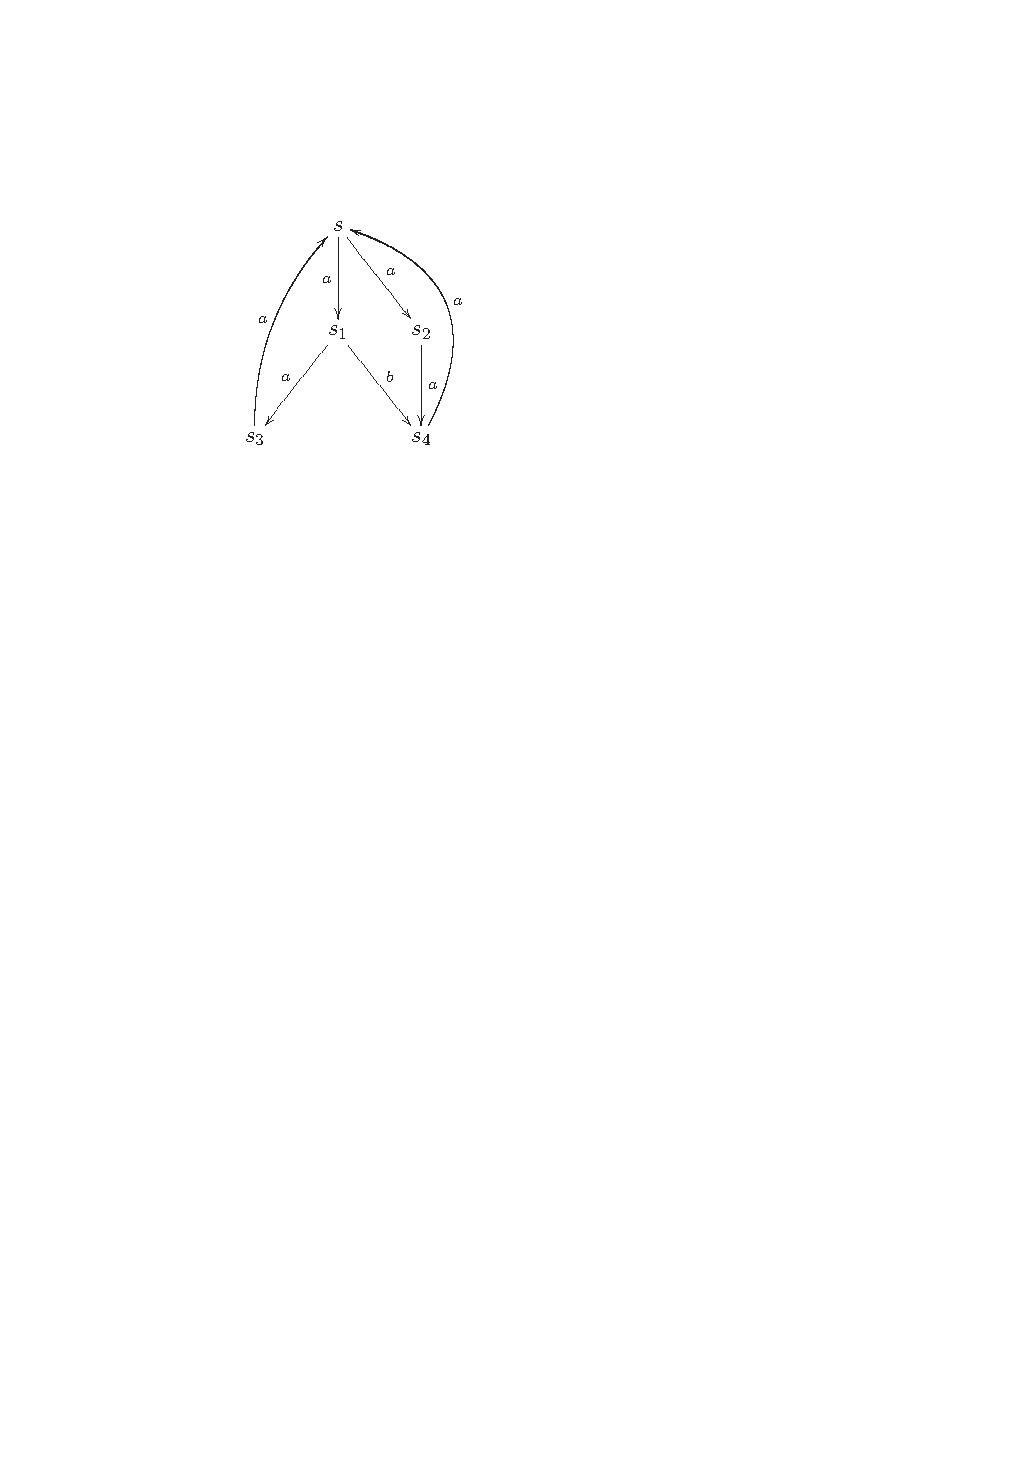
\includegraphics{images/LTS-1}
}{\centering
  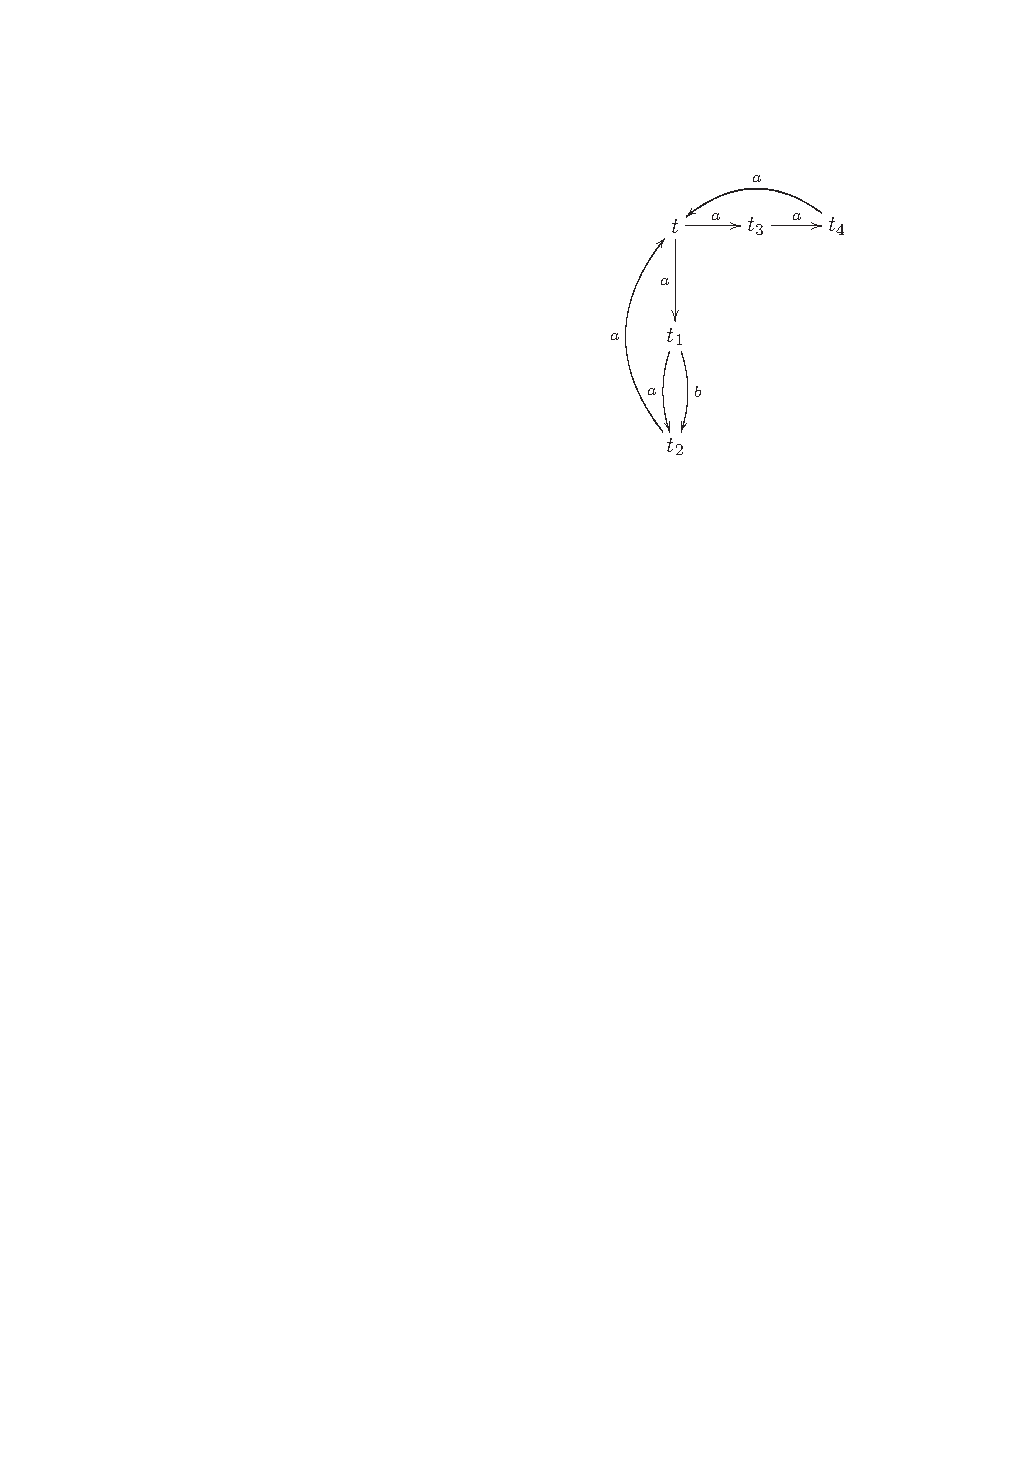
\includegraphics{images/LTS-2}
}
\end{exampleblock}
\end{slide}
%Rania Khalaf (IBM T.J. Watson Research Center, USA) - rkhalaf@us.ibm.com	

%-------------------------------------------------------------------------------
\begin{slide}{More bisimulations}
\small

\myblock{Considering $\tau$-transitions}

\begin{block}{Weak transition}
\begin{align*}
  p \Trans{\alpha} q ~~~&\text{iff}~~~
  p \,(\rtran{\tau})^{*}\, q_1\rtran{a} q_2 \,(\rtran{\tau})^{*}\, q
  \\
  p \Trans{\tau} q ~~~&\text{iff}~~~
  p \,(\rtran{\tau})^{*}\, q
\end{align*}  
where $\alpha \neq \tau$ and $(\rtran{\tau})^{*}$ is the reflexive and transitive closure of $\rtran{\tau}$.
\end{block}

\begin{block}{Weak bisimulation (vs. strong)}
Given  $\pair{S_1, \Act,  \rra_1}$  and $\pair{S_2, \Act, \rra_2}$ over $\Act$,
relation $R \subseteq S_1 \times S_2$ is a \structure{bisimulation} iff for all $\pair{p,q} \in R$ and $a \in \Act\,\rdb{\cup \set{\tau}}$,
%
\begin{align*}
%\text{\alert{(1)}}\; \;  &  p \downarrow_1 \;  \dimp\; q \downarrow_2\\ &\\
\text{\alert{(1)}}\; \;  & p \rtran{a}_1 p'\; \imp\;
  \rcb{\exists}{q'}{q' \in S_2}{\rdb{q \Trans{a}_2  q'}\, \e\,
  \pair{p',q'} \in R}   \\
\text{\alert{(2)}}\; \;  & q \rtran{a}_2 q'\; \imp\;
  \rcb{\exists}{p'}{p' \in S_1}{\rdb{p \Trans{a}_1 p'}\, \e\,
  \pair{p',q'} \in R}   
\end{align*}
%\centering
%\begin{tikzpicture}[%
%    every edge/.style={draw, thick,-latex',shorten >= 2pt}]
%  \tikzstyle{l} = [auto,inner sep=1pt]
%  % the square
%  \node(p){$p$};\node[right=2.3 of p](q2){$q$};
%  \node[below=1 of p](p'){$p'$};\node(q')at(p'-|q2){$q'$};
%  % the R parts
%  \node[right=0 of p](R1){$R$};\node[right=0 of R1](q){$q$};
%  \node[left=0 of q'](R2){$R$};\node[left=0 of R2](p'2){$p'$};
%  % the arrows
%  \draw[->] (p)edge node[l]{$a$}(p') (q2)edge node[l]{$a$}(q');
%  \node at ($(p)!.5!(q')$){{\Large $\Rightarrow$}};
%  %%%%%%%
%  % the square
%  \node[right=2.3 of q2](pp){$p$};\node[right=2.3 of pp](q2){$q$};
%  \node[below=1 of pp](p'){$p'$};\node(q')at(p'-|q2){$q'$};
%  % the R parts
%  \node[right=0 of p'](R1){$R$};\node[right=0 of R1](q){$q'$};
%  \node[left=0 of q2](R2){$R$};\node[left=0 of R2](p'2){$p$};
%  % the arrows
%  \draw[->] (pp)edge node[l]{$a$}(p') (q2)edge node[l]{$a$}(q');
%  \node at ($(pp)!.5!(q')$){{\Large $\Leftarrow$}};
%\end{tikzpicture}
\end{block}
\end{slide}



\begin{slide}{More bisimulations}
\small
\myblock{Considering $\tau$-transitions}


\begin{block}{Branching bisimulation}
Given  $\pair{S_1, \Act,  \rra_1}$  and $\pair{S_2, \Act, \rra_2}$ over $\Act$,
relation $R \subseteq S_1 \times S_2$ is a \structure{bisimulation} iff for all $\pair{p,q} \in R$ and $a \in \Act\,\rdb{\cup\set{\tau}}$,
%
\begin{align*}
%\text{\alert{(1)}}\; \;  &  p \downarrow_1 \;  \dimp\; q \downarrow_2\\ &\\
&\text{\alert{(1)} if}\; \;   p \rtran{a}_1 p'\; \text{then either}
  \\&~~
  \text{\alert{(1.1)}~} a=\tau \text{~and~}\pair{p',q}\in R \text{~~or}
  \\&~~
  \text{\alert{(1.2)}~}
    \rcb{\exists}{q',q'' \in S_2}{}{\rdb{q \,(\trans{\tau}_2)^{*}\,q' \tran{a}_2  q''}\, \e\,
    \pair{p,q'} \in R \e\,
    \pair{p',q''} \in R} \\[3mm]
%&\text{\alert{(2)} if}\; \;   q \rtran{a}_2 q'\; \imp\;
%  \rcb{\exists}{p'}{p' \in S_1}{\rdb{p \Trans{a}_1 p'}\, \e\,
%  \pair{p',q'} \in R}   
&\text{\alert{(2)} if}\; \;   q \rtran{a}_2 q'\; \text{then either}
  \\&~~
  \text{\alert{(2.1)}~} a=\tau \text{~and~}\pair{p',q'}\in R \text{~~or}
  \\&~~
  \text{\alert{(2.2)}~}
    \rcb{\exists}{p',p'' \in S_1}{}{\rdb{p \,(\trans{\tau}_1)^{*}\,p' \tran{a}_1  p''}\, \e\,
    \pair{p',q} \in R \e\,
    \pair{p'',q'} \in R}
\end{align*}
\end{block}
\end{slide}

%-------------------------------------------------------------------------------
%
%\begin{slide}{mCRL2}
%  
%\begin{itemize}
%  \item {Formal \structure{specification language} with an associated toolset}
%  
%  \item {Used for \structure{modelling}, \structure{validating} and \structure{verifying} concurrent systems and protocols}
%\end{itemize}
%  
%\end{slide}
%
%-------------------------------------------------------------------------------
%
%\begin{slide}{mCRL2 - toolset overview}
%\centering  
%
%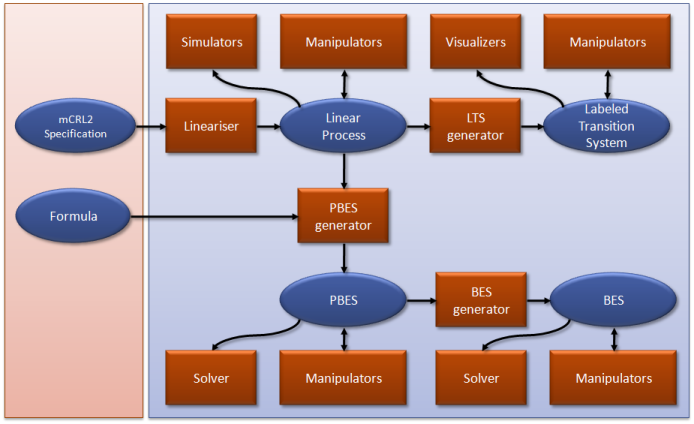
\includegraphics[width=.9\textwidth]{images/mcrl2-toolset}
%  
%\end{slide}
%
%-------------------------------------------------------------------------------

\end{document}

